\documentclass[french,paper=a4,oneside,captions=tableheading]{article}

%% Language and font encodings
\usepackage[french]{babel}
\usepackage[utf8x]{inputenc}
\usepackage[T1]{fontenc}

%% Useful packages
\usepackage{graphicx}
\usepackage[colorinlistoftodos]{todonotes}
\PassOptionsToPackage{hyphens}{url}
\usepackage[colorlinks=true, allcolors=black]{hyperref}
\usepackage{longtable}

%% Pour changer la police
\usepackage[default]{sourcesanspro}

%% Pour la page de garde
\usepackage{pagecolor}
\usepackage{afterpage}
\usepackage[margin=2.5cm,includehead=true,includefoot=true,centering]{geometry}

%% Pour les exemples
\usepackage{mdframed}
\newmdenv[topline=false, bottomline=false, rightline=false, skipabove=\topsep, skipbelow=\topsep]{example}

%% Tikz
\usepackage{pgf-pie}
\usepackage{tikz}
\usetikzlibrary{backgrounds}
\pgfkeys{/donut/.cd,
inner radius/.initial=3.14cm,
inner radius=3.14cm,
outer radius/.initial=2cm,
outer radius=2cm,
text color/.initial=white,
text color=white}
\newcommand{\donutchart}[2][]{
   % Calculate total
   \pgfmathsetmacro{\totalnum}{0}
   \foreach [count=\n] \value/\colour/\name in {#2} {
     \pgfmathparse{\value+\totalnum}
     \global\let\totalnum=\pgfmathresult
     \xdef\numitems{\n}
   }

  \begin{tikzpicture}
  \pgfmathsetmacro{\wheelwidth}{\pgfkeysvalueof{/donut/outer
  radius}-\pgfkeysvalueof{/donut/inner radius}}
  \pgfmathsetmacro{\midradius}{(\pgfkeysvalueof{/donut/outer radius}
  +\pgfkeysvalueof{/donut/inner radius})/2}

  \begin{scope}[#1]

    \pgfmathsetmacro{\cumnum}{0}
    \foreach \value/\colour/\name in {#2} {
        \pgfmathsetmacro{\newcumnum}{\cumnum + \value/\totalnum*360}

        \pgfmathsetmacro{\midangle}{-(\cumnum+\newcumnum)/2}
        \begin{scope}[on background layer]
          \filldraw[draw=white,fill=\colour]
          (-\cumnum:\pgfkeysvalueof{/donut/outer radius}) 
           arc(-\cumnum:-(\newcumnum):\pgfkeysvalueof{/donut/outer radius}) --
          (-\newcumnum:\pgfkeysvalueof{/donut/inner radius}) 
          arc(-\newcumnum:-(\cumnum):\pgfkeysvalueof{/donut/inner radius}) -- cycle;
        \end{scope}
        \draw node [text=\pgfkeysvalueof{/donut/text color}, 
        font=\bfseries\sffamily] at 
        (\midangle:{\pgfkeysvalueof{/donut/inner radius}+\wheelwidth/2}) {\value \%};

        \global\let\cumnum=\newcumnum
    }
    
    \node[text width=\textwidth] at (-4,0) {
        \foreach \value/\colour/\name in {#2} {
           {\color{\colour}\textbullet}\space\name \hfill
        }    
    };
    
    \node at (0,0) {Vulnérabilités};
    
  \end{scope}

  \end{tikzpicture}}

% variables for title, author and date
\usepackage{titling}
\title{Pentest des infrastructures de MegaCorpOne}
\author{Grégoire Roumache - Maxime Wallemme}
\date{21-12-2021}

%% header & footer
\usepackage[headsepline,footsepline]{scrlayer-scrpage}
\newpairofpagestyles{header-footer}{
  \clearpairofpagestyles
  \ihead[21-12-2021]{\raisebox{1ex}{Pentest des infrastructures de MegaCorpOne}}
  \chead[]{}
  \ohead[Pentest des infrastructures de MegaCorpOne]{\raisebox{1ex}{21-12-2021}}
  \ifoot[\thepage]{\raisebox{-1ex}{Grégoire Roumache - Maxime Wallemme}}
  \cfoot[]{}
  \ofoot[Grégoire Roumache - Maxime Wallemme]{\raisebox{-1ex}{\thepage}}
  \addtokomafont{pageheadfoot}{\upshape}
}
\pagestyle{header-footer}


%% To list and caption code
\usepackage{minted}
\renewcommand{\listoflistingscaption}{Table des programmes}
\usepackage{caption}
\newenvironment{code}{\captionsetup{type=listing}}{}
\renewcommand{\listingscaption}{Programme}



\begin{document}




\begin{titlepage}
    \newgeometry{left=6cm}
    \definecolor{titlepage-color}{HTML}{1E90FF}
    \newpagecolor{titlepage-color}\afterpage{\restorepagecolor}
    \newcommand{\colorRule}[3][black]{\textcolor[HTML]{#1}{\rule{#2}{#3}}}
    \begin{flushleft}
        \noindent
        \\[-1em]
        \color[HTML]{FFFAFA}
        \makebox[0pt][l]{\colorRule[FFFAFA]{1.3\textwidth}{2pt}}
        \par
        \noindent
        {
          \vfill
          \noindent {\huge \textbf{\textsf{Pentest des infrastructures de MegaCorpOne}}}
            \vskip 1em
          {\Large \textsf{Rapport de pentest}}
            \vskip 2em
          \noindent {\Large \textsf{Grégoire Roumache - Maxime Wallemme}}
          \vfill
        }
        \textsf{21 Décembre 2021}
    \end{flushleft}
\end{titlepage}

\let\cleardoublepage\clearpage

\tableofcontents \newpage



\begin{center}
\section*{Historique des versions}
\addcontentsline{toc}{section}{Historique des versions}
\end{center}

\begin{table}[h]
    \centering
    \begin{tabular}{|l|c|l|}
        \hline
        Date du document & Version & Description des changements \\
        \hline
        21-12-2021 & 1.0 & Version initiale \\
        \hline
    \end{tabular}
\end{table}


\cleardoublepage
\newpage








\section{Résumé}

Nous avons reçu la tâche de réaliser un pentest des infrastructures de MegaCorpOne. Un pentest est une méthode d'évaluation de la sécurité d'un système d'information par la simulation d'attaques similaires à celles réalisées par des hackers dont l'objectif serait d'infiltrer MegaCorpOne. Les objectifs de ce test étaient d'identifier les infrastructures informatiques de l'entreprise et les failles qu'elles possèdent, de les exploiter, ainsi que de proposer des solutions pour les combler.

Lors de la réalisation de ce pentest, nous avons trouvés plusieurs vulnérabilités critiques dans le système d'information de MegaCorpOne. Nous avons pu accéder à plusieurs machines du réseau de l'entreprise et ce, avec un accès administrateur. Ceci est dû principalement à des configurations de sécurité faibles, des applications qui ne sont pas à jour et une politique de mots de passe trop faible.

Voici une liste des systèmes et le niveau d'accès que nous avons pu obtenir :

\begin{center} \begin{tabular}{llll}
    Adresse IP    & Nom d'hôte               & Système d'exploitation & Niveau d'accès            \\ \hline
    10.180.20.1   & Sovkipou.ptlab.be        & Windows 2016           & Administrateur du domaine \\
    10.180.20.2   & Soporifik.ptlab.be       & Windows 2003           & Administrateur            \\
    10.180.20.3   & Simiabraz.ptlab.be       & Windows 10             & Administrateur            \\
    10.180.20.11  & /                        & Linux                  & /                         \\
    10.180.30.10  & Snubbull.megacorpone.eu  & Linux                  & Accès root \\
    10.180.30.15  & Stalgamin.megacorpone.be & Linux                  & /                         \\
\end{tabular} \end{center}
Les adresses IP 10.180.20.254 et 10.180.30.254 étaient aussi utilisées mais ce sont les adresses des routeurs des sous-réseaux que nous avons attaqués.

Et voici la liste des service que nous avons découverts sur ces machines :

\begin{center} \begin{longtable}{llllp{8.5cm}}
    Adresse IP   & Port & Protocol & Nom & Informations complémentaires  \\ \hline
    10.180.20.1  & 21    & tcp & ftp          & Microsoft ftpd \\
    10.180.20.1  & 53    & tcp & domain       & Simple DNS Plus \\
    10.180.20.1  & 80    & tcp & http         & Microsoft IIS httpd 10.0 \\
    10.180.20.1  & 88    & tcp & kerberos-sec & Microsoft Windows Kerberos server time: 2021-12-01 14:59:21Z \\
    10.180.20.1  & 135   & tcp & msrpc        & Microsoft Windows RPC \\
    10.180.20.1  & 139   & tcp & netbios-ssn  & Microsoft Windows netbios-ssn \\
    10.180.20.1  & 389   & tcp & ldap         & Microsoft Windows Active Directory LDAP Domain: ptlab.be, Site: Default-First-Site-Name \\
    10.180.20.1  & 445   & tcp & microsoft-ds & Windows Server 2016 Datacenter 14393 microsoft-ds workgroup: PTLAB \\
    10.180.20.1  & 464   & tcp & kpasswd5     & / \\
    10.180.20.1  & 593   & tcp & ncacn\_http  & Microsoft Windows RPC over HTTP 1.0 \\
    10.180.20.1  & 636   & tcp & ssl/ldap     & Microsoft Windows Active Directory LDAP Domain: ptlab.be, Site: Default-First-Site-Name \\
    10.180.20.1  & 3268  & tcp & ldap         & Microsoft Windows Active Directory LDAP Domain: ptlab.be, Site: Default-First-Site-Name \\
    10.180.20.1  & 3269  & tcp & ssl/ldap     & Microsoft Windows Active Directory LDAP Domain: ptlab.be, Site: Default-First-Site-Name \\
    10.180.20.1  & 3389  & tcp & ms-wbt-server& Microsoft Terminal Services \\
    10.180.20.1  & 5985  & tcp & http         & Microsoft HTTPAPI httpd 2.0 SSDP/UPnP \\
    10.180.20.1  & 9389  & tcp & mc-nmf       & .NET Message Framing \\
    10.180.20.1  & 49666 & tcp & msrpc        & Microsoft Windows RPC \\
    10.180.20.1  & 49667 & tcp & msrpc        & Microsoft Windows RPC \\
    10.180.20.1  & 49685 & tcp & ncacn\_http  & Microsoft Windows RPC over HTTP 1.0 \\
    10.180.20.1  & 49686 & tcp & msrpc        & Microsoft Windows RPC \\
    10.180.20.1  & 49688 & tcp & msrpc        & Microsoft Windows RPC \\
    10.180.20.1  & 49708 & tcp & msrpc        & Microsoft Windows RPC \\
    10.180.20.1  & 49719 & tcp & msrpc        & Microsoft Windows RPC \\
    10.180.20.1  & 49960 & tcp & msrpc        & Microsoft Windows RPC \\
    10.180.20.2  & 139   & tcp & netbios-ssn  & Microsoft Windows netbios-ssn \\
    10.180.20.2  & 445   & tcp & microsoft-ds & Windows XP 3790 Service Pack 1 microsoft-ds workgroup: PTLAB \\
    10.180.20.3  & 135   & tcp & msrpc        & Microsoft Windows RPC \\
    10.180.20.3  & 139   & tcp & netbios-ssn  & Microsoft Windows netbios-ssn \\
    10.180.20.3  & 445   & tcp & microsoft-ds & / \\
    10.180.20.3  & 5040  & tcp & unknown      & / \\
    10.180.20.3  & 49664 & tcp & msrpc        & Microsoft Windows RPC \\
    10.180.20.3  & 49665 & tcp & msrpc        & Microsoft Windows RPC \\
    10.180.20.3  & 49666 & tcp & msrpc        & Microsoft Windows RPC \\
    10.180.20.3  & 49667 & tcp & msrpc        & Microsoft Windows RPC \\
    10.180.20.3  & 49668 & tcp & msrpc        & Microsoft Windows RPC \\
    10.180.20.3  & 49669 & tcp & msrpc        & Microsoft Windows RPC \\
    10.180.20.3  & 49670 & tcp & msrpc        & Microsoft Windows RPC \\
    10.180.20.3  & 49671 & tcp & msrpc        & Microsoft Windows RPC \\
    10.180.20.11 & 5555  & tcp & freeciv      & / \\
    10.180.30.10 & 22    & tcp & ssh          & OpenSSH 6.6.1p1 Ubuntu 2ubuntu2.13 Ubuntu Linux; protocol 2.0 \\
    10.180.30.10 & 80    & tcp & http         & Apache httpd 2.4.7 (Ubuntu) \\
    10.180.30.15 & 22    & tcp & ssh          & OpenSSH 8.4p1 Debian 5 protocol 2.0 \\
    10.180.30.15 & 80    & tcp & http         & nginx 1.18.0    \\
    10.180.30.15 & 111   & tcp & rpcbind      & 2-4 RPC \#100000 \\
    10.180.30.15 & 443   & tcp & ssl/http     & nginx 1.18.0    \\
    10.180.30.15 & 2049  & tcp & nfs\_acl     & 3 RPC \#100227   \\
    10.180.30.15 & 36175 & tcp & mountd       & 1-3 RPC \#100005 \\
    10.180.30.15 & 39589 & tcp & mountd       & 1-3 RPC \#100005 \\
    10.180.30.15 & 43065 & tcp & nlockmgr     & 1-4 RPC \#100021 \\
    10.180.30.15 & 56001 & tcp & mountd       & 1-3 RPC \#100005 \\
\end{longtable} \end{center}















\section{Recommendations}

Nous recommandons de patcher les vulnérabilités identifiés lors de ce test et de renforcer la politique de mots de passe. Une fois ces tâches effectuées, nous pensons qu'il faut s'assurer qu'un attaquant ne pourra plus exécuter ces attaques en effectuant des tests. Il faudra aussi faire attention aux nouvelles vulnérabilités qui ne manqueront pas d'arriver dans le futur et continuer de protéger les systèmes au quotidien avec une stratégie de patching régulière.















\section{Méthodologie utilisée}

Nous avons utilisé une méthode souvent pratiquée par les hackers expérimentés pour s'attaquer à une entreprise. Elle est divisée en plusieurs étapes en commençant par la recherche d'informations sur l'entreprise afin de découvrir des vulnérabilités. Une fois trouvées, il faut les exploiter pour rentrer dans le système informatique de l'entreprise. Et finalement, on se déplace dans le système en attaquant d'autres machines de l'infrastructure et en essayant de prendre le contrôle de comptes administrateur.















\subsection{Cadre du pentest}

Dans le cadre de ce pentest, il a été décidé préalablement de chercher des informations pouvant conduire à une attaque de phishing ciblée mais de ne pas conduire cette attaque pour se concentrer sur l'aspect technique du système d'information. Concrètement, cela veut dire que nous avons réuni des informations sur les réseaux sociaux pour pouvoir nous faire passer pour un employé, comme le font certains hackers, afin de faire du social engineering mais nous n'avons pas conduit cette attaque.










\subsection{Reconnaissance}

Lors de cette étape très importante du pentest, nous avons cherché un maximum d'informations sur l'entreprise qui peuvent être utiles à des hackers dont l'objectif est de nuire à l'entreprise. L'objectif est de trouver et comprendre la surface d'attaque de l'entreprise autant d'un point de vue technique comme trouver le nombre de serveurs, domaines et sous-domaines internet; que des données qui pourraient être utiles à des fins de social engineering, comme des informations sur le CEO ou d'autres employés de l'entreprise. Ceci, sans outil de scan et énumération.



\subsubsection{Informations sur quelques employés de la société}

\begin{enumerate}
    \item CEO, Joe Sheer:
    \begin{itemize}
        \item né en 1968,
        \item twitter: \url{https://twitter.com/joe\_sheer/},
        \item email: \url{joe@megacorpone.com}.
    \end{itemize}
    \item Personne de contact technique (IT and Security Director), Alan Grofield:
    \begin{itemize}
        \item travaille chez MegaCorp One depuis 1983,
        \item linkedin: \url{https://www.linkedin.com/in/alan-grofield-32806468},
        \item email: \url{agrofield@megacorpone.com}.
    \end{itemize}
    \item Recruteur, Handy McKay:
    \begin{itemize}
        \item twitter: \url{https://twitter.com/McKayHandy}.
    \end{itemize}
    \item Stagiaire, William Adler:
    \begin{itemize}
        \item twitter: \url{https://twitter.com/RealWillAdler}.
    \end{itemize}
    \item WEB designer, Tom Hudson:
    \begin{itemize}
        \item email: \url{thudson@megacorpone.com},
        \item twitter: \url{https://twitter.com/TomHudsonMCO}.
    \end{itemize}
    \item Développeur senior (Senior Developper), Tanya Rivera:
    \begin{itemize}
        \item email: \url{trivera@megacorpone.com},
        \item twitter: \url{https://twitter.com/TanyaRiveraMCO}.
    \end{itemize}
    \item Directeur marketing (Marketing Director), Matt Smith:
    \begin{itemize}
        \item email: \url{msmith@megacorpone.com},
        \item twitter: \url{https://twitter.com/MattSmithMCO}.
    \end{itemize}
    \item Vice-président des affaires juridiques (VP Of Legal), Mike Carlow:
    \begin{itemize}
        \item email: \url{mcarlow@megacorpone.com},
        \item linkedin: \url{https://www.linkedin.com/in/mike-carlow-8128896a/}.
    \end{itemize}
\end{enumerate}



\subsubsection{Informations sur le nom de domaine}

\begin{enumerate}
    \item Date d'enregistrement du nom de domaine:
    \begin{itemize}
        \item 22-01-2013
    \end{itemize}
    \item Sous-domaines de megacorpone:
    \begin{itemize}
        \item admin.megacorpone.com
        \item beta.megacorpone.com
        \item fs1.megacorpone.com
        \item ftp.megacorpone.com
        \item intranet.megacorpone.com
        \item mail.megacorpone.com
        \item mail2.megacorpone.com
        \item manager.megacorpone.com
        \item mgmt.megacorpone.com
        \item michael.megacorpone.com
        \item ns1.megacorpone.com
        \item ns2.megacorpone.com
        \item ns3.megacorpone.com
        \item remote.megacorpone.com
        \item router.megacorpone.com
        \item siem.megacorpone.com
        \item snmp.megacorpone.com
        \item support.megacorpone.com
        \item svn.megacorpone.com
        \item syslog.megacorpone.com
        \item test.megacorpone.com
        \item vpn.megacorpone.com
        \item webmail.megacorpone.com
        \item www.megacorpone.com
        \item www2.megacorpone.com
    \end{itemize}
\end{enumerate}



\subsubsection{Informations sur le serveur WEB et les serveurs DNS}

\begin{enumerate}
    \item Hébergeur:
    \begin{itemize}
        \item OVH
    \end{itemize}
    \item Pays d'hébergement du site web:
    \begin{itemize}
        \item Montréal, Québec, Canada
    \end{itemize}
    \item Adresse IP publique du site web:
    \begin{itemize}
        \item 149.56.244.87
    \end{itemize}
    \item Changement d'hébergement du site web:
    \begin{itemize}
        \item Le site web n'a pas changé d'hébergement. Le statut du transfert de client est sur "interdit" (clientTransferProhibited). \cite{1}
    \end{itemize}
    \item Operating system du site web: Debian 10
    \item Technologie du web server: apache/2.4.38
    \item Vulnérabilités connues pour la version du web server:
    \begin{itemize}
        \item CVE-2018-17189: DoS for HTTP/2 connections via slow request bodies (low)
        \item CVE-2018-17199: mod\_session\_cookie does not respect expiry time (low)
        \item CVE-2019-0190: mod\_ssl 2.4.37 remote DoS when used with OpenSSL 1.1.1 (important)
    \end{itemize}
    \item Technologies web utilisées: PHP/7.3.29-1
    \item Name servers de la société:
    \begin{itemize}
        \item ns1.megacorpone.com
        \item ns2.megacorpone.com
        \item ns3.megacorpone.com
    \end{itemize}
\end{enumerate}



\subsubsection{Informations sensibles}

\begin{enumerate}
    \item Hash du mot de passe de l'utilisateur trivera, trouvé sur le github de l'entreprise:
    \begin{itemize}
        \item hash: \texttt{trivera{}:\$apr1\$A0vSKwao\$GV3sgGAj53j.c3GkS4oUC0}
        \item commande utilisée pour trouver le mot de passe à partir du hash: \texttt{john -{}-wordlist=rockyou.txt hash.txt}
        \item résultat: \texttt{trivera{}:Tanya4life}
    \end{itemize}
    
    \item Informations sur l'utilisateur William Adler:
    Nous supposons qu'il pourrait s'agir des identifiants de l'utilisateur pouvant lui servir à accéder à l'un des services interne de l'entreprise.
    \begin{itemize}
        \item Nom d'utilisateur: Wadler
        \item Mot de passe: TwitterStar2
        \item Informations trouvées sur le twitter de l'employé William Adler (Voir figure \ref{SensitiveInformations})
    \end{itemize}
    \begin{figure}[H]
        \centering
        
\includegraphics[width=15cm]{images/InformationSensibleWilliamAdler.png}
        \caption{Informations sensibles de l'utilisateur William Adler}
        \label{SensitiveInformations}
    \end{figure}
\end{enumerate}



\subsubsection{Autres informations}

\begin{enumerate}
    \item Adresse de l'entreprise: 2 Old Mill St, 89001 Rachel, Nevada US.
    \item Numéro de téléphone: +1.9038836342.
    \item Adresses mail des différents départements:
    \begin{itemize}
        \item département des ressources humaines (Human Resources): \url{hr@megacorpone.com},
        \item département commercial (Sales): \url{sales@megacorpone.com},
        \item département logistique (Shipping): \url{shipping@megacorpone.com}.
    \end{itemize}
    \item Réseaux sociaux de l'entreprise:
    \begin{itemize}
        \item facebook (contenu indisponible): \url{https://www.facebook.com/MegaCorp-One-393570024393695/}
        \item linkedin (contenu indisponible): \url{https://www.linkedin.com/company/18268898/}
        \item github: \url{https://github.com/megacorpone}
    \end{itemize}
    \item Format d'adresses mails de la société:
    \begin{itemize}
        \item Employés: 1ère lettre du prénom + nom de famille + @megacorpone.com
        \item Département: Initiales ou nom complet du département + @megacorpone.com
        \item PDG: Prénom + @megacorpone.com
    \end{itemize}
    \item Page web non référencée: \url{https://www.megacorpone.com/nanites.php}
    \item Page web anciennement référencées:
    \begin{itemize}
        \item \url{http://www.megacorpone.com/jobs2.html}
        \item \url{https://cp.megacorpone.net/}
    \end{itemize}
\end{enumerate}










\subsection{Scanning et énumération}

Le scanning et l'énumération est la deuxième étape du pentest, elle s'inscrit dans la continuité de l'étape de reconnaissance parce qu'elle continue la recherche d'informations sur l'entreprise mais avec une différence majeure: l'utilisation d'outils de scanning automatisés. L'objectif est de trouver un maximum d'informations sur les services informatiques de l'entreprise accessibles depuis l'extérieur. Par exemple, nous avons scanné le site web de MegaCorpOne pour trouver des pages intéressantes comme une partie du site réservée aux administrateurs.



\subsubsection{Identification des adresses IP d'intérêt}

À l'aide des commandes \texttt{ping} et \texttt{nslookup}, nous avons trouvé deux adresses IP d'intérêt:
\begin{enumerate}
    \item l'adresse du serveur WEB: 10.180.30.15,
    \item et l'adresse du serveur DNS: 10.180.20.1.
\end{enumerate}

Ensuite, nous avons énuméré les enregistrements DNS avec la commande \texttt{dnsenum megacorpone.be}, dont voici le résultat:
\begin{example}
\begin{Verbatim}
megacorpone.be.             3600     IN    SOA               (
megacorpone.be.             3600     IN    NS       sovkipou.ptlab.be.
Stalgamin.megacorpone.be.   3600     IN    A        10.180.30.15
www.megacorpone.be.         3600     IN    CNAME    Stalgamin.megacorpone.be.
\end{Verbatim}
\end{example}

Malheureusement, ça n'a pas donné de résultats importants. Nous connaissons aussi notre adresses IP grâce à la commande \texttt{ip address}, c'est l'adresse IPv4 10.180.10.1. Nous avons aussi une adresse IPv6 unicast mais pas d'adresse IPv6 globale.



\subsubsection{Scanning du réseau}

Nous avons décidé de scanner les réseaux contenant les serveurs WEB (10.180.30.15/24) et DNS (10.180.20.1/24) comme vous pouvez le voir sur la figure \ref{fig:NetworkScan}. C'est ainsi que nous avons trouvé que 8 hôtes étaient présents sur ces réseaux. Voici leurs IP:
\begin{itemize}
    \item 10.180.30.10
    \item 10.180.30.15
    \item 10.180.30.254
    \item 10.180.20.1
    \item 10.180.20.2
    \item 10.180.20.3
    \item 10.180.20.11
    \item 10.180.20.254
\end{itemize}

\begin{figure}[H]
    \centering
    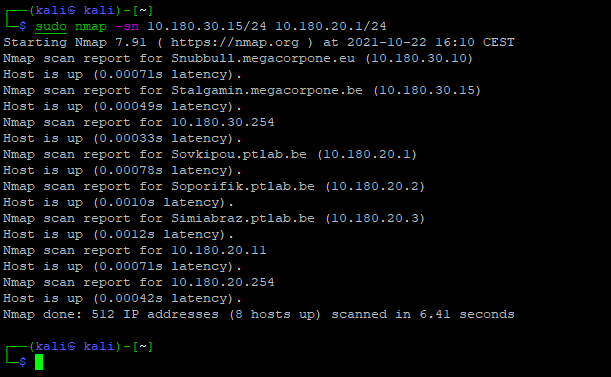
\includegraphics[width=15cm]{images/Secu_Offensive_10.png}
    \caption{Scan des réseaux contenant les serveurs WEB (10.180.30.15/24) et DNS (10.180.20.1/24)}
    \label{fig:NetworkScan}
\end{figure}



\subsubsection{Nmap - TCP scanning}

Dans cette partie, nous scannons les ports des adresses \texttt{10.180.20.1} et \texttt{10.180.30.15} à l'aide des commandes:
\begin{itemize}
    \item \texttt{sudo nmap -sS 10.180.20.1}
    \item \texttt{sudo nmap -sT 10.180.20.1}
    \item \texttt{sudo nmap -sS 10.180.30.15}
    \item \texttt{sudo nmap -sT 10.180.30.15}
\end{itemize}
L'option \texttt{-sS} est utilisée pour exécuté un scan TCP SYN. Cela permet d'effectuer un scan rapide et peu bruyant car il n'établit pas entièrement une connexion TCP. Car il envoie un paquet SYN qui attends alors une réponse:
\begin{itemize}
    \item SYN/ACK : Le port est ouvert
    \item RST : Le port est fermé
    \item Si aucune réponse après plusieurs essais : Le port est filtré
\end{itemize}

L'option \texttt{-sT} elle est utilisée pour exécuté un scan TCP connect. Contrairement à l'option \texttt{-sS}, celle-ci est moins efficace et n'est utilisée que lorsque le SYN ne peut-être utilisé, ce qui est le cas lorsque l'utilisateur ne possède pas les privilèges nécessaires ou lorsqu'il s'agit d'un scan IPv6. Avec cette option, Nmap demande à l'OS d'établir une connexion au port de la machine cible à l'aide de l'appel système \texttt{connect()}.



\subsubsection{Nmap - UDP scanning}

Pour effectuer le scan, nous forçons l'utilisation de UDP par Nmap à l'aide de l'option \texttt{-sU}. La commande utilisée est celle-ci: \\

\texttt{sudo nmap -sU 10.180.20.1 10.180.30.15}\\
Comme on peut le voir sur la figure \ref{fig:Scan_UDP_Nmap}, le résultat obtenu montre que le port 53, 111, 2049 et 49262 sont ouverts.

\begin{figure}[H]
    \centering
    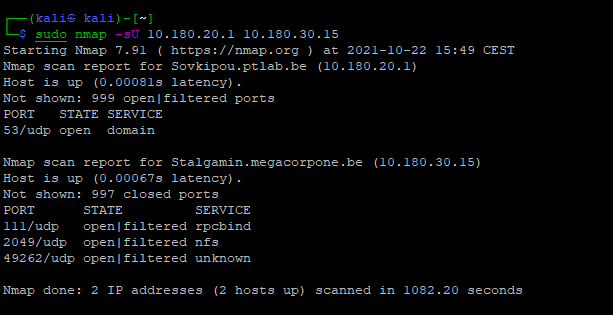
\includegraphics[width=16cm]{images/Secu_Offensive_9.png}
    \caption{Résultat du scan UDP avec Nmap}
    \label{fig:Scan_UDP_Nmap}
\end{figure}



\subsubsection{OS Fingerprinting}

Maintenant, nous allons lancer un scan pour déterminer les systèmes d'exploitation de ces machines. Ça peut être accompli facilement avec l'option -O de nmap. Voici donc la commande utilisée: \texttt{sudo nmap -O 10.180.30.10 10.180.30.15 10.180.30.254 10.180.20.1 10.180.20.2 10.180.20.3 10.180.20.11 10.180.20.254}, \\ dont voici le résultat:
\begin{itemize}
    \item 10.180.30.10:  Linux 3.2 - 4.9
    \item 10.180.30.15:  Linux 4.15 - 5.6
    \item 10.180.30.254: Linux 4.15 - 5.6
    \item 10.180.20.1:   Microsoft Windows Server 2016
    \item 10.180.20.2:   Microsoft Windows Server 2003 SP1 or SP2, Microsoft Windows Server 2003 SP2, Microsoft Windows Server 2008 Enterprise SP2
    \item 10.180.20.3:   Microsoft Windows 10 1709 - 1909
    \item 10.180.20.11:  Linux 4.15 - 5.6
    \item 10.180.20.254: Linux 4.15 - 5.6
\end{itemize}



\subsubsection{Banner Grabbing/Service Enumeration}

Ensuite, nous avons lancé l'énumération des services sur ces huit machines avec l'option -sV qui sert à déterminer la nature des services tournant sur la machine ainsi que leurs versions. Voici ce que nous avons trouvés avec la commande: \\
\texttt{sudo nmap -sV 10.180.30.10 10.180.30.15 10.180.30.254 10.180.20.1 10.180.20.2 10.180.20.3} \\ \texttt{10.180.20.11 10.180.20.254}
\begin{center}
    \begin{tabular}{|c|c|c|c|} \hline
        \textbf{IP}   & \textbf{Port} & \textbf{Service} & \textbf{Version}  \\ \hline \hline
        10.180.30.10  & 2049          & nfs              & 3-4 (RPC \#100003) \\ \hline
        10.180.30.15  & /             & /                & /                 \\ \hline
        10.180.30.254 & /             & /                & /                 \\ \hline
        10.180.20.1   & /             & /                & /                 \\ \hline
        10.180.20.2   & 139           & netbios-ssn      & /                 \\
                      & 445           & microsoft-ds     & /                 \\ \hline
        10.180.20.3   & /             & /                & /                 \\ \hline
        10.180.20.11  & /             & /                & /                 \\ \hline
        10.180.20.254 & /             & /                & /                 \\ \hline
    \end{tabular}
\end{center}



\subsubsection{Nmap Scripting Engine (NSE)}

L'outil de scanning de ports nmap contient aussi des scripts qui peuvent être utilisés pour nous fournir encore plus d'informations. Pour en exécuter un, on utilise la syntaxe suivante: \texttt{sudo nmap -{}-script=<script> <hôtes>}. Voici les résultats pour quelques-uns de ces scripts:
\begin{itemize}

\item smb-os-discovery
\begin{example}
\begin{Verbatim}
Nmap scan report for Sovkipou.ptlab.be (10.180.20.1)

Host script results:
| smb-os-discovery: 
|   OS: Windows Server 2016 Datacenter 14393 (Windows Server 2016 Datacenter 6.3)
|   Computer name: Sovkipou
|   NetBIOS computer name: SOVKIPOU\x00
|   Domain name: ptlab.be
|   Forest name: ptlab.be
|   FQDN: Sovkipou.ptlab.be
|_  System time: 2021-10-22T16:22:19+02:00
\end{Verbatim}
\end{example}
\hspace{0.3cm}
\begin{example}
\begin{Verbatim}
Nmap scan report for Soporifik.ptlab.be (10.180.20.2)

Host script results:
| smb-os-discovery: 
|   OS: Windows XP 3790 Service Pack 1 (Windows XP 5.2)
|   Computer name: Soporifik
|   NetBIOS computer name: SOPORIFIK\x00
|   Domain name: ptlab.be
|   Forest name: ptlab.be
|   FQDN: Soporifik.ptlab.be
|_  System time: 2021-10-22T16:22:18+02:00
\end{Verbatim}
\end{example}

\item vuln, voir la figure \ref{fig:vuln}.

\begin{figure}[H]
    \centering
    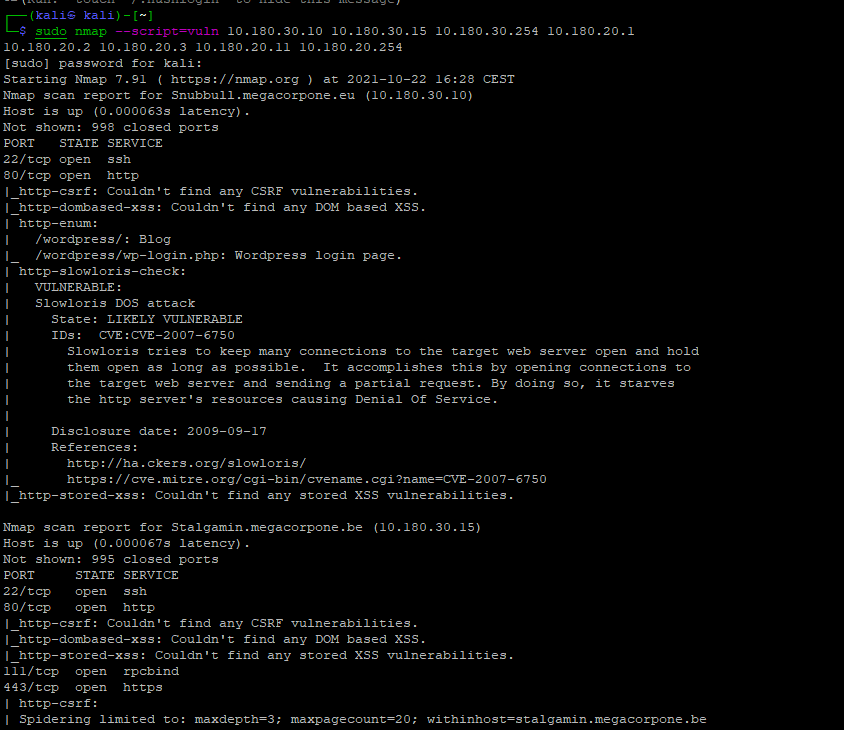
\includegraphics[width=15cm]{images/Secu_Offensive_17.png}
    \caption{Partie 1 -- Résultat du scan de vulnérabilités avec nmap}
    \label{fig:vuln}
\end{figure}
\begin{figure}[H]\ContinuedFloat
    \centering
    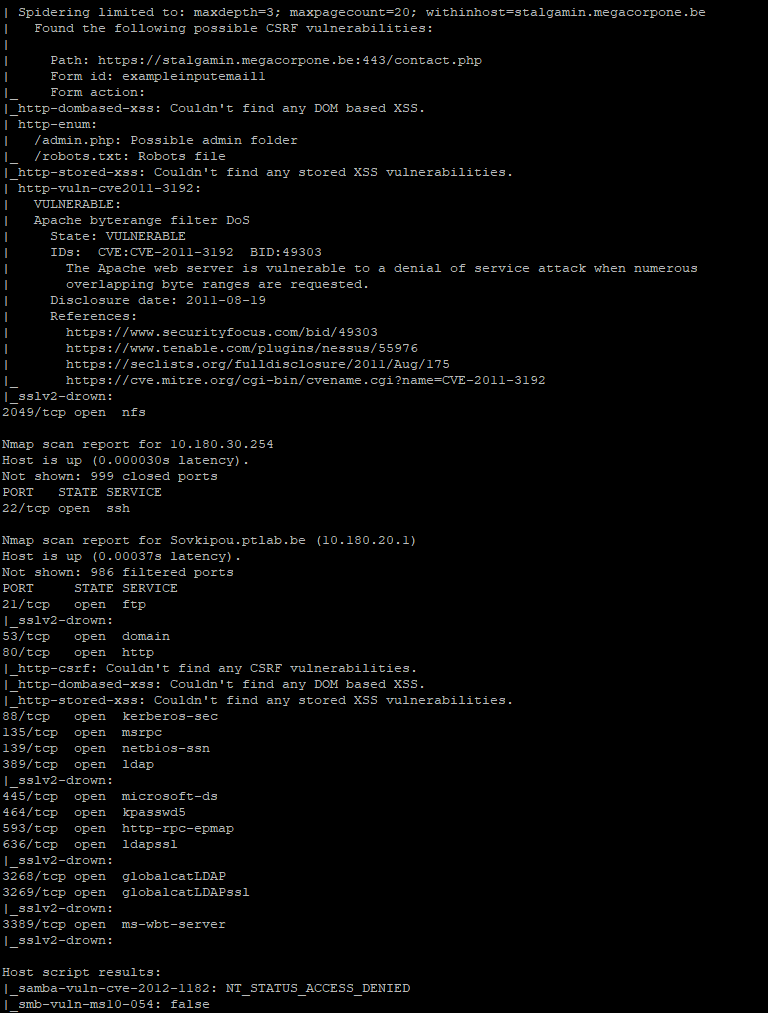
\includegraphics[width=14cm]{images/Secu_Offensive_18.png}
    \caption{Partie 2 -- Résultat du scan de vulnérabilités avec nmap}
    \label{fig:vuln}
\end{figure}
\begin{figure}[H]\ContinuedFloat
    \centering
    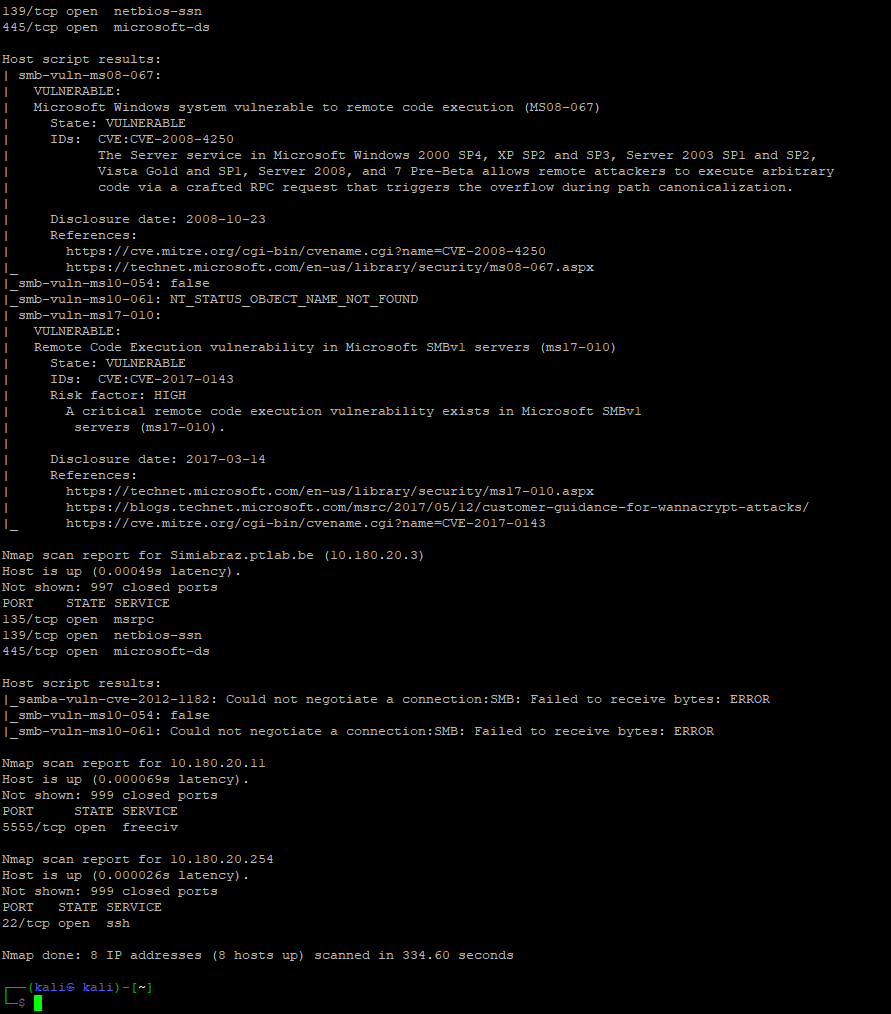
\includegraphics[width=16cm]{images/Secu_Offensive_19.png}
    \caption{Partie 3 -- Résultat du scan de vulnérabilités avec nmap}
    \label{fig:vuln}
\end{figure}

\end{itemize}



\subsubsection{SMB Enumeration}

Grâce aux scans précédents, nous savons qu'il n'y a qu'une IP avec un service SMB: 10.180.20.2. Nous allons lancer plusieurs scans sur cette adresse. Vous pouvez voir ces scans sur les figures \ref{fig:smb1}, \ref{fig:smb2}, \ref{fig:smb3}, \ref{fig:smb4}, \ref{fig:smb5}.

\begin{figure}[H]
    \centering
    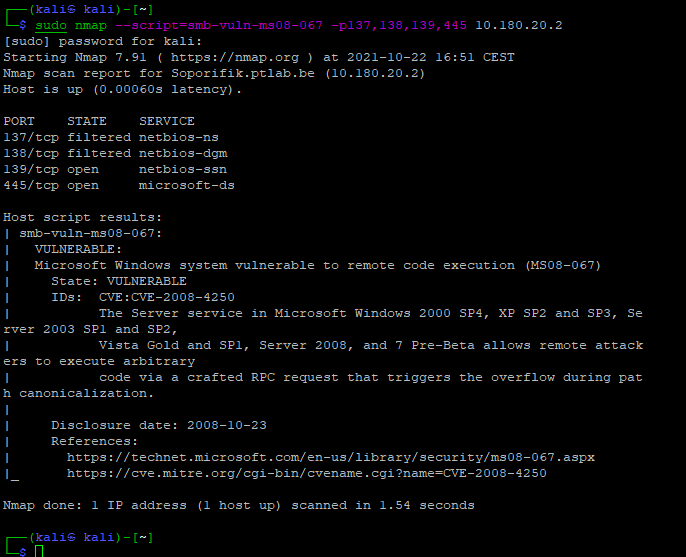
\includegraphics[width=15cm]{images/Secu_Offensive_20.png}
    \caption{Scan smb-vuln-ms-08-067}
    \label{fig:smb1}
\end{figure}

A l'aide de ce scan, nous pouvons observé que la machine est vulnérable à la faille smb-vuln-ms08-067. Celle-ci rend la machine sous Windows vulnérable à une attaque permettant l'exécution de code.

\begin{figure}[H]
    \centering
    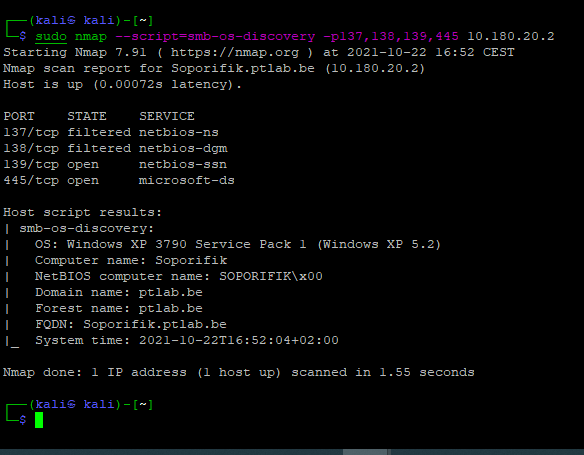
\includegraphics[width=13cm]{images/Secu_Offensive_21.png}
    \caption{Scan smb-os-discovery}
    \label{fig:smb2}
\end{figure}

Nous pouvons ici obtenir l'OS présent sur la machine. Il s'agit de Windows XP. Mais aussi, nous pouvons observé le nom de l'ordinateur ainsi que le nom du domaine dans lequel il se trouve.

\begin{figure}[H]
    \centering
    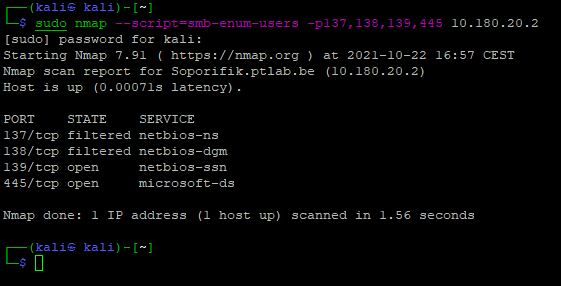
\includegraphics[width=11cm]{images/Secu_Offensive_22.png}
    \caption{Scan smb-enum-users}
    \label{fig:smb3}
\end{figure}

Nous n'avons obtenu aucun utilisateurs présents sur la machine.

\begin{figure}[H]
    \centering
    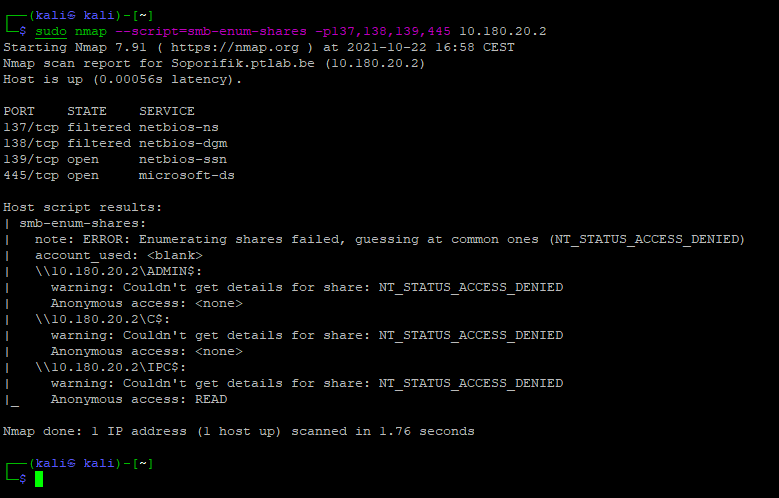
\includegraphics[width=15cm]{images/Secu_Offensive_23.png}
    \caption{Scan smb-enum-shares}
    \label{fig:smb4}
\end{figure}

Nous pouvons ici observé différents dossiers partagés présents sur la machine à l'aide du script \textit{smb-enum-shares}

\begin{figure}[H]
    \centering
    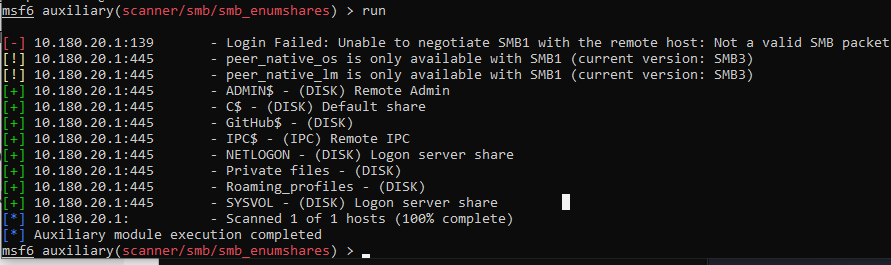
\includegraphics[width=16cm]{images/smb-shares-enum-msf.png}
    \caption{Scan d'énumération des shares smb avec metasploit sur l'IP 10.180.20.1}
    \label{fig:smb-shares-enum-msf}
\end{figure}

Ensuite, à l'aide de metasploit et du module smb\_enumshares, nous avons pu confirmé les dossiers partagés présents dans le scan nmap. Mais aussi découvrir de nouveaux dossiers.

\begin{figure}[H]
    \centering
    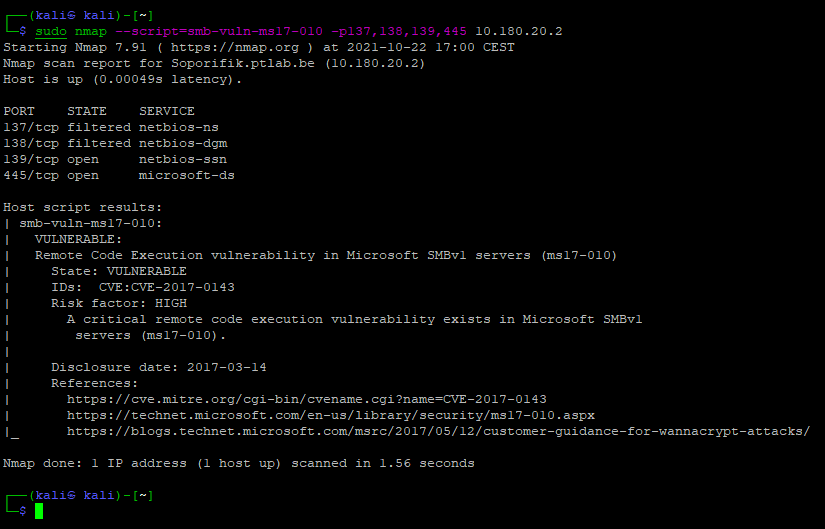
\includegraphics[width=15cm]{images/Secu_Offensive_24.png}
    \caption{Scan smb-vuln-ms17-010}
    \label{fig:smb5}
\end{figure}

A l'aide du script nmap \textit{smb-vumn-ms17-010}, nous savons que la machine est vulnérable à la faille smb-vuln-ms17-010. Cette dernière permettant l'exécution de code à distance sur la machine.

\subsubsection{NFS Enumeration}

Nous avons effectués les scans nfs-showmount, nfs-ls, nfs-statfs, et voici les informations que nous en tirons:
\begin{itemize}
    \item NFS tourne sur le serveur avec l'adresse: 10.180.30.15
    \item Le montage suivant est présent sur le serveur: /srv/nfs-shared 10.180.0.0/16
    \item Voici les permissions sur ce dossier: rwx r-x r-x
    \item Dans ce dossier, il y a un fichier hello.txt dont les permissions sont: rw- -{}-{}- -{}-{}-
    \item Voici l'usage de ce dossier sur le disque:
\begin{example}
\begin{Verbatim}
nfs-statfs: 
  Filesystem      1K-blocks  Used      Available  Use% Maxfilesize Maxlink
  /srv/nfs-shared 15421320.0 1544492.0 13071660.0 11%  16.0T       32000
\end{Verbatim}
\end{example}
    \item En montant ce dossier partagé sur notre machine avec la commande: \\
    \texttt{sudo mount -t nfs 10.180.30.15:/srv/nfs-shared /mnt -o nolock} \\
    nous pouvons lire le fichier mais il ne contient pas d'informations intéressantes, seulement ceci:
\begin{example}
\begin{Verbatim}
Hello World!
\end{Verbatim}
\end{example}
\end{itemize}



\subsubsection{SNMP Enumeration}

Pour ce qui est de l'énumération du protocole SNMP, nous avons utilisés à la fois les scripts nmap et snmpwalk (voir figure \ref{fig:snmpwalk}).

\begin{figure}[H]
    \centering
    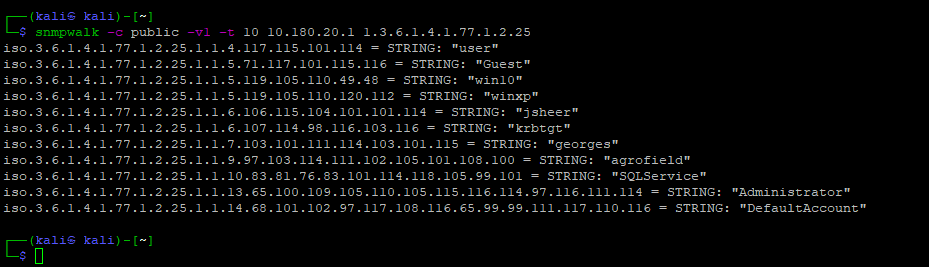
\includegraphics[width=17cm]{images/Secu_Offensive_35.png}
    \caption{Trouver les utilisateurs avec snmpwalk}
    \label{fig:snmpwalk}
\end{figure}

Pour ce qui est des scripts nmap, nous avons utilisés ceux-ci:
\begin{itemize}

\item snmp-win32-users
\begin{example}
\begin{Verbatim}
snmp-win32-users: 
  Administrator
  DefaultAccount
  Guest
  SQLService
  agrofield
  georges
  jsheer
  krbtgt
  user
  win10
  winxp
\end{Verbatim}
\end{example}

\item snmp-win32-shares
\begin{example}
\begin{Verbatim}
snmp-win32-shares
  SYSVOL: C:\Windows\SYSVOL\sysvol
  NETLOGON: C:\Windows\SYSVOL\sysvol\ptlab.be\SCRIPTS
  Private files: C:\Private files
  Roaming_profiles: C:\Roaming_profiles
\end{Verbatim}
\end{example}

\item snmp-win32-software, qui ne nous donne pas des informations très intéressantes pour l'exploitation de la machine. En effet, après avoir lancé ce scan, nous savons qu'il y a Microsoft Visual C++, VMware Tools et rien de plus.

\end{itemize}



\subsubsection{WEB Enumeration}

Enfin, pour ce qui est de l'énumération WEB, nous avons utilisé l'outil dirb avec cette commande ci: \texttt{dirb http://10.180.30.10/ /usr/share/wordlists/dirb/big.txt}. Les résultats de ce scan sont montrés sur la figure \ref{fig:dirb}.

\begin{figure}[H]
    \centering
    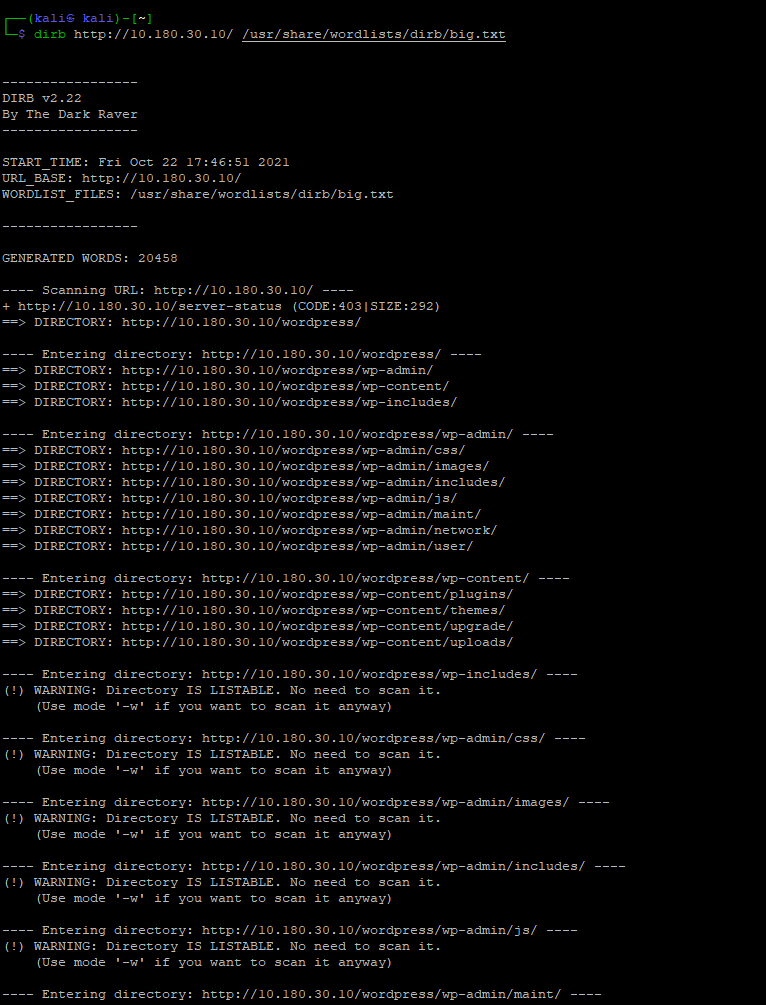
\includegraphics[width=15cm]{images/Secu_Offensive_38.png}
    \caption{Partie 1 -- Résultat du scan WEB avec dirb}
    \label{fig:dirb}
\end{figure}
\begin{figure}[H]\ContinuedFloat
    \centering
    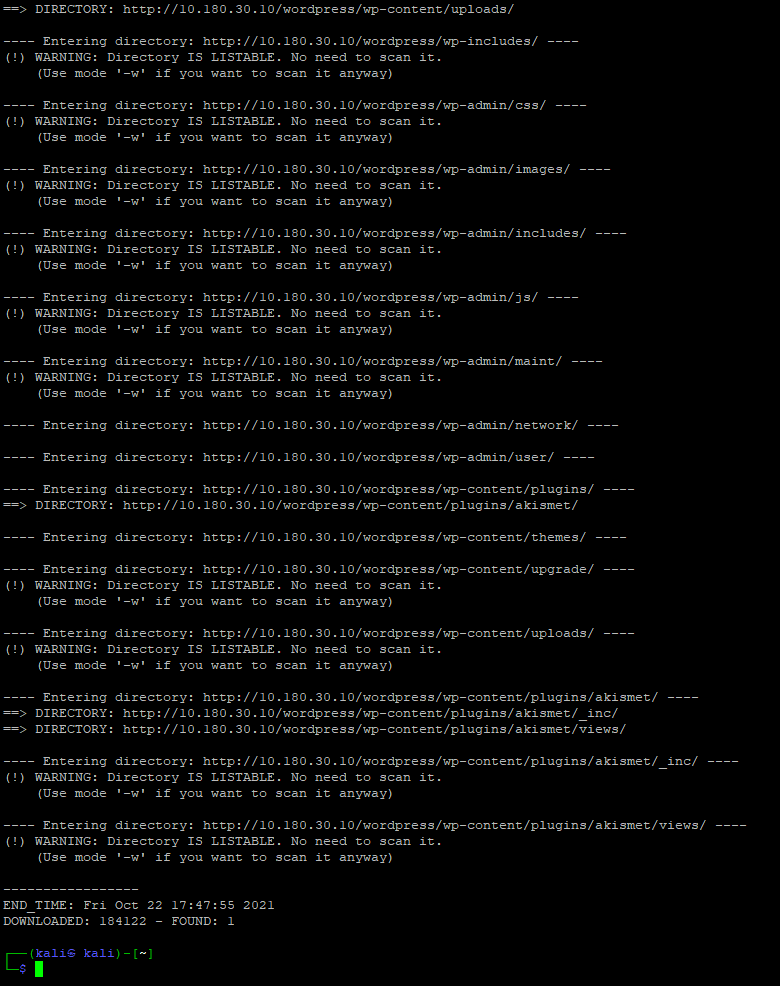
\includegraphics[width=16cm]{images/Secu_Offensive_39.png}
    \caption{Partie 2 -- Résultat du scan WEB avec dirb}
    \label{fig:dirb}
\end{figure}



\subsubsection{Wordpress Enumeration}

Étant donné la présence d'un site Wordpress sur la machine 10.180.30.10, nous avons lancés un scan Wordpress (figure \ref{fig:wordpress-scan}) qui nous a permis de découvrir les thèmes et extensions utilisés comme \textit{slideshow-gallery}.

\begin{figure}[H]
    \centering
    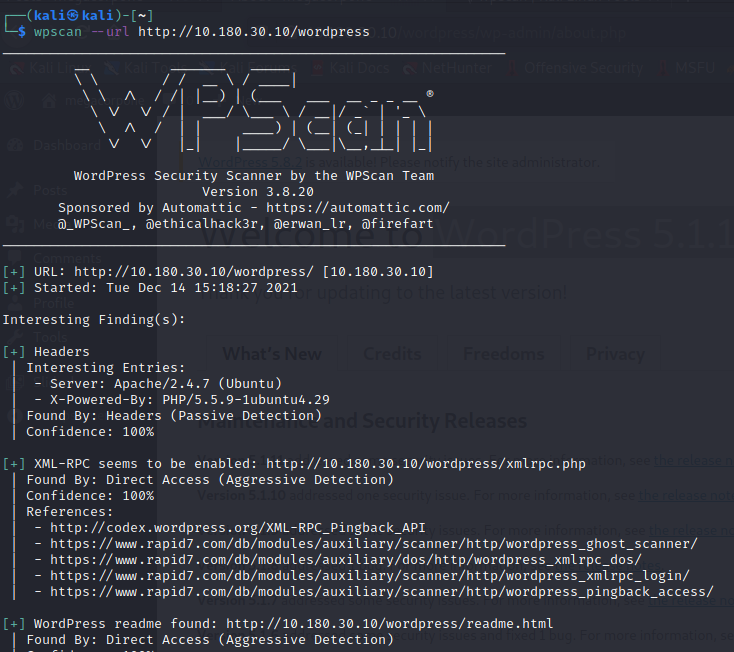
\includegraphics[width=16cm]{images/wordpress-scan.png}
    \caption{Scan Wordpress avec wpscan}
    \label{fig:wordpress-scan}
\end{figure}












\subsection{Analyse de vulnérabilités}



\subsubsection{Nessus}

Afin de réaliser certains scans de vulnérabilités, nous avons utilisés le logiciel Nessus. Ce dernier offre la possibilité de réaliser différents types de scans sur une infrastructure et notamment des scans de vulnérabilités. Dans notre cas, nous l'avons utilisés pour la recherche de vulnérabilités sur différentes machines, ainsi qu'un scan web.



\subsubsection{Types de vulnérabilités}

Voici les différents types de vulnérabilités trouvés, on remarque que les scores les plus élevés comme Critical, High et Medium sont présents en grand nombre.

\donutchart[rotate=90]{16.7/purple/CRITICAL,23.3/red/HIGH,50/orange/MEDIUM,10/yellow/LOW}



\subsubsection{Scan - 10.180.20.1}

Le scan nous retourne différentes vulnérabilités pouvant être présentes sur le système possédant l'ip 10.180.20.1 .\\
\textbf{Vulnérabilités de type HIGH :}
\begin{itemize}
    \item 7.5 - SSL Medium Strength Cipher Suites Supported (SWEET32) \\
\textbf{Description :}
Le protocole SSL utilise un cryptage de force moyenne. Il est plus facile de contourner un niveau de cryptage de force moyenne lorsqu'on se trouve dans le même réseau physique.

\textbf{CVE :}
CVE-2016-2183

\textbf{Solution :}
Afin de contrer cette vulnérabilité, il faut procéder à une reconfiguration pour utiliser un cryptage avec un niveau plus élevé.\\

    \item Hydra:FTP \\
\textbf{Description :}
Lors de la configuration du scan, nous avons utiliser l'option de bruteforce sur le service FTP. Nessus retourne le résultat que le mot de passe FTP peut être découvert à l'aide d'une méthode de brute force.

\textbf{Solution :}
Changer les mots de passe des comptes affectés.

\textbf{Résultat :}
La méthode de brute force lancée par Nessus nous a retournée un nom d'utilisateur et un mot de passe.\\
Username : user\\
Password : Tigrou007\\

    \item SNMP Agent Default Community Name \\
\textbf{Description :}
Le nom de communauté par défaut du serveur SNMP peut être obtenu. A l'aide de ce nom, un attaquant peut l'utiliser afin d'obtenir plus d'information sur l'hôte ou modifier la configuration du système.

\textbf{CVE :}
CVE-1999-0517

\textbf{Solution :}
Il existe différentes solutions pour contrer le problème de cette vulnérabilité:
\begin{enumerate}
    \item Désactiver le service SNMP
    \item Changer le nom de communauté par défaut
    \item Filtrer les paquets UDP entrants vers le port 161
\end{enumerate}

    \item Microsoft Windows SMB Shares Unprivileged Access \\
\textbf{Description :}
Il est possible d'accéder à certains dossiers partagés sur le serveur distant.

\textbf{Solution :}
Restreint l'accès aux dossiers partagés. \\

\begin{figure}[H]
    \centering
    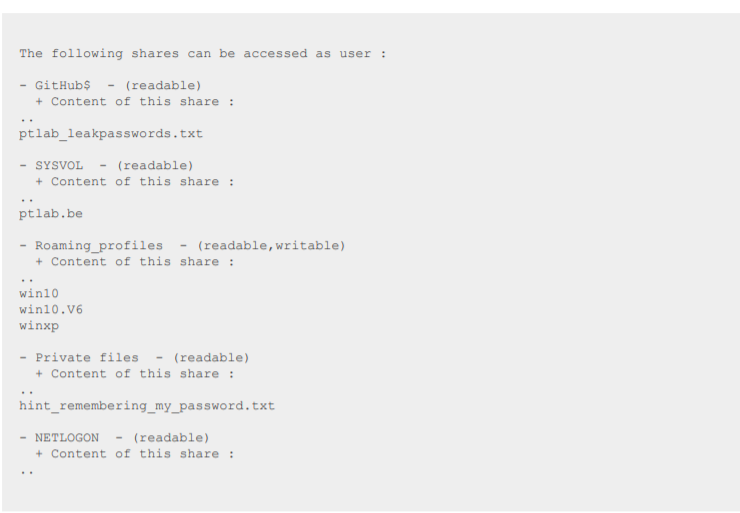
\includegraphics[width=11cm]{images/sharefolder.png}
    \caption{Dossiers partagés accessibles avec le user correspondant}
    \label{fig:sharefolder}
\end{figure}

\end{itemize}

\textbf{Vulnérabilités de type MEDIUM :}
\begin{itemize}
    \item SSL Certificate Cannot Be Trusted\\
\textbf{Description :}
Le certificat SSL de l'hôte ne peut être approuvé.Plus loins dans l'analyse, on remarque que Nessus à détecté un certificat auto signé ce qui justifie cette vulnérabilité.

\textbf{Solution :}
Il faut générer un certificat SSL approprié et valide.\\

\item TLS Version 1.0 Protocol Detection\\
\textbf{Description :}
Le service TLS 1.0 utilisé, chiffre le trafic avec des ressources cryptographiques non recommandées.

\textbf{Solution :}
Utiliser une version TLs plus récente, TLS 1.2 ou 1.3.\\

\item SSL RC4 Cipher Suites Supported\\
\textbf{Description :}
RC4 est pris en charge par l'hôte dans une ou plusieurs suites de chiffrement. RC4 possède un défaut de chiffrement diminuant son caractère aléatoire. Si RC4 est utilisé à plusieurs reprises pour le chiffrement du texte en clair (ex: cookies), alors l'attaquant en récupérant plusieurs textes chiffrés pourrait être en mesure de déchiffrer le texte en clair.

\textbf{CVE :}
CVE-2013-2566\\
CVE-2015-2808

\textbf{Solution :}
Eviter l'utilisation du chiffrement via RC4. Utiliser TLS 1.2.\\

\item DNS Server Zone Transfer Information Disclosure\\
\textbf{Description :}
Le DNS permet d'utiliser des transferts de zone DNS. Cela permettrait à un attaquant de récupérer des informations sensibles pour réaliser des recherches approfondies sur l'infrastructure de sa cible.

\textbf{CVE :}
CVE-1999-0532

\textbf{Solution :}
Limiter le transfert de zone DNS uniquement aux serveurs ayant besoin des informations.\\
\end{itemize}

\textbf{Information :}
\begin{itemize}
    \item OS identification\\
Le système d'exploitation utiliser par l'hôte serait Windows 10 selon l'analyse faite par Nessus.\\

    \item Microsoft Windows 'Administrators' Group User List \\
Lors du scan Credential Patch Audit, Nessus à pu récupérer une petite liste de groupes et utilisateurs que voici : 

\begin{figure}[H]
    \centering
    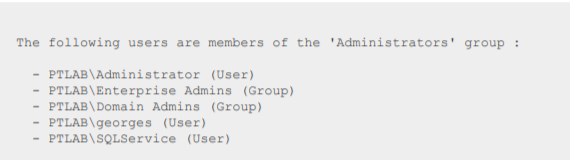
\includegraphics[width=11cm]{images/users_admingroup.png}
    \caption{Liste d'utilisateurs et groupes}
    \label{fig:userlist}
\end{figure}
    
    \item Microsoft Windows SAM user enumeration \\
Nessus à trouvé des noms d'utilisateurs dans le SAM. Le SAM est un fichier de base de données présent sur les systèmes Windows Server 2003, Windows XP et Windows 2000.

\begin{figure}[H]
    \centering
    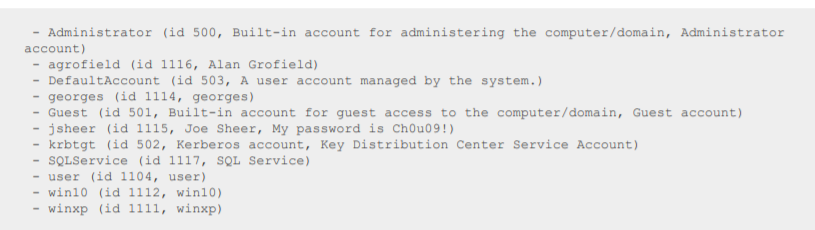
\includegraphics[width=11cm]{images/userSAM.png}
    \caption{Liste d'utilisateurs du SAM}
    \label{fig:userlistSAM}
\end{figure}

\end{itemize}



\subsubsection{Scan - 10.180.20.2}

Le scan retourne différentes vulnérabilités pouvant être présentes sur le système ayant l'ip 10.180.20.2 . \\

\textbf{Vulnérabilités de type CRITICAL :}
\begin{itemize}
    \item MS08-067: Microsoft Windows Server Service Crafted RPC Request
Handling Remote Code Execution\\
\textbf{Description :}
L'hôte windows est affecté par une vulnérabilité permettant d'exécuter du code à distance à cause d'une mauvaise gestion des requêtes RPC. Un attaquant peut utiliser cette faille à l'aide d'une requête forgée RPC pour exécuter du code sans être authentifié.

\textbf{CVE :}
CVE-2008-4250

\textbf{Solution :}
Mettre à jour le système, Microsoft à sorti une série de patch concernant cette faille.\\

\item MS06-040: Vulnerability in Server Service Could Allow Remote Code
Execution \\
\textbf{Description :}
L'hôte distant est vulnérable à un buffer overflow dans le service Server. Un attaquant pourrait exécuter du code arbitraire à distance avec les privilèges SYSTEM.

\textbf{CVE :}
CVE-2006-3439

\textbf{Solution :}
Mettre à jour le système, Microsoft à sorti une série de patch concernant cette faille.\\

\item MS09-001: Microsoft Windows SMB Vulnerabilities Remote Code Execution \\
\textbf{Description :}
Une vulnérabilité de corruption de mémoire présente dans SMB permettant à un attaquant d'exécuter du code arbitraire ou de réaliser un DOS contre l'hôte distant.

\textbf{CVE :}
CVE-2008-4834 \\
CVE-2008-4835 \\
CVE-2008-4114

\textbf{Solution :}
Mettre à jour le système, Microsoft à sorti une série de patch concernant cette faille.\\
\end{itemize}

\textbf{Vulnérabilités de type HIGH :}\\
\begin{itemize}
\item MS17-010: Security Update for Microsoft Windows SMB Server \\
\textbf{Description :}
De multiples vulnérabilités permettant d'exécuter du code à distance existe dans SMBv1.

\textbf{CVE :}
CVE-2017-0143 \\
CVE-2017-0144\\
CVE-2017-0145\\
CVE-2017-0146\\
CVE-2017-0147\\
CVE-2017-0148


\textbf{Solution :}
Mettre à jour le système, Microsoft à sorti une série de patch concernant cette faille.\\

\item Microsoft Windows SMB NULL Session Authentication \\
\textbf{Description :}
Il est possible pour un attaquant de se connecter à l'hôte distant à l'aide d'une session NULL, c'est à dire sans login ou mot de passe.

\textbf{CVE :}
CVE-1999-0519\\
CVE-1999-0520\\
CVE-2002-1117


\textbf{Solution :}
Effectuer des modifications dans les registres.\\

\end{itemize}

\textbf{Vulnérabilités de type MEDIUM :}\\
\begin{itemize}
    \item Microsoft Windows EFSRPC NTLM Reflection Elevation of Privilege \\

\textbf{Description :}
L'hôte distant est affecté par une vulnérabilité d'élévation de privilèges de réflexion NTLM.

\textbf{CVE :}
CVE-2021-36942

\textbf{Solution :}
Effectuer les mises à jour fournies par le vendeur.

    \item SMB Signing not required \\
\textbf{Description :}
Une signature n'est pas requise sur le serveur SMB distant. Un attaquant non authentifié peut exploiter cette faille à distance.

\textbf{Solution :}
Appliquer la signature des messages dans la configuration de l'hôte.\\

\end{itemize}

\textbf{Information :}\\

\begin{itemize}
    \item OS Identification\\
Nessus à identifié l'hôte comme étant une machine Windows 5.1 soit une machine sous WindowsXP.\\

    \item Microsoft Windows SAM user enumeration
Nessus à pu trouver l'utilisateur \textit{\textbf{Administrator}}
\end{itemize}



\subsubsection{Scan - 10.180.20.3}

Le scan retourne différentes vulnérabilités pouvant être présentes sur le système ayant l'ip 10.180.20.3 . \\
\textbf{Vulnérabilités de type MEDIUM :}\\



\begin{itemize}
    \item SMB Signing not required \\
\textbf{Description :}
Une signature n'est pas requise sur le serveur SMB distant. Un attaquant non authentifié peut exploiter cette faille à distance.

\textbf{Solution :}
Appliquer la signature des messages dans la configuration de l'hôte.\\

\end{itemize}

\textbf{Information :}\\

\begin{itemize}
    \item OS Identification\\
Nessus à identifié l'hôte comme étant une machine sous Windows 10 Pro.
\end{itemize}



\subsubsection{Scan - 10.180.30.10}

Le scan retourne différentes vulnérabilités pouvant être présentes sur le système ayant l'ip 10.180.30.10 .\\
\textbf{Vulnérabilités de type HIGH :}\\
\begin{itemize}
    \item CGI Generic SQL Injection \\
\textbf{Description :}
Nessus à détecté qu'une page était potentiellement vulnérable à une injection SQL. 

\begin{figure}[H]
    \centering
    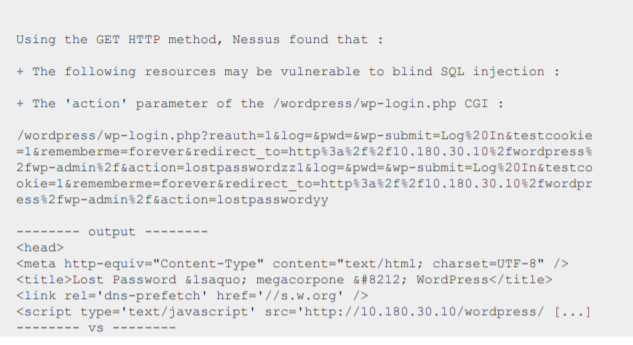
\includegraphics[width=11cm]{images/injection_sql.png}
    \caption{Page potentiellement vulnérable à une injection SQL}
    \label{fig:sqlinjection}
\end{figure}

\end{itemize}


\textbf{Vulnérabilités de type MEDIUM :}\\

\begin{itemize}
    \item Browsable Web Directories \\
\textbf{Description :}
Plusieurs répertoires du serveur web sont consultables depuis le site internet.

\textbf{Solution :}
S'assurer que les répertoires ne contiennent pas d'informations sensibles. Utiliser des restrictions d'accès ou désactiver l'indexation des répertoires.\\

    \item SSH Weak Algorithms Supported \\
\textbf{Description :}
Le serveur SSH est configuré pour accepter des algorithmes de cryptages faibles ou aucun algorithmes.

\textbf{Solution :}
Supprimer les chiffrements faibles.\\

    \item Web Application Potentially Vulnerable to Clickjacking\\
\textbf{Description :}
Le site est potentiellement vulnérable au clickjacking ce qui permettrait à un attaquant de faire cliquer un utilisateur sur une zone de la page web vulnérable et différente de ce que l'utilisateur peut voir.

\textbf{Solution :}
Que la page renvoie dans sa réponse l'en-tête Content-Security-Policy.\\

    \item WordPress User Enumeration \\
\textbf{Description :}
La version Wordpress du serveur web contient une vulnérabilité pouvant aider un attaquant non authentifié à lister le nom des utilisateurs Wordpress. \\
Nessus à retourné dans ses résultats deux noms d'utilisateurs:
\begin{itemize}
    \item wordpressuser
    \item blogger
\end{itemize} \hspace{0.2cm}

    \item mDNS Detection \\
\textbf{Description :}
Le service possède le protocole mDNS qui permet de découvrir des informations sur l'hôte distant comme l'OS et sa version, le nom d'hôte et les services qu'il exécute.

\textbf{Solution :}
Filtrer le trafic entrant vers le port UDP 5353.\\

\end{itemize}

\textbf{Vulnérabilités de type LOW :}\\

\begin{itemize}
    \item SSH Weak Key Exchange Algorithms Enabled\\
\textbf{Description :}
SSH est configuré pour accepter des algorithmes d'échange de clés faibles.

\textbf{Solution :}
Désactiver les algorithmes faibles.\\

    \item Web Server Allows Password Auto-Completion\\
\textbf{Description :}
Le serveur web contient au moins un formulaire HTML avec une entrée de mot de passage où l'autocomplétion est activé. Ce qui signifie que les données d'identification d'un utilisateur peuvent être enregistrées dans son navigateur. Si la machine d'un utilisateur est compromise, il pourrait facilement accéder à ces données d'identification.

\textbf{Solution :}
Désactiver l'option d'autocomplétion sur le serveur web.\\

    \item Web Server Transmits Cleartext Credentials
\textbf{Description :}
Plusieurs champs de formulaire HTML de type mot de passe transmettent leurs informations en texte clair. Un attaquant espionnant le réseau pourrait obtenir les identifiants et mot de passe d'utilisateurs.

\textbf{Solution :}
S'assurer que les informations soient transmises via HTTPS.\\

\end{itemize}

\textbf{Information :} \\

\begin{itemize}
    \item Apache HTTP Server Version\\
Nessus a détecté dans son scan que la version Apache utilisée est la 2.4.99\\

    \item OS Identification\\
Le serveur web se trouve sur une machine Ubuntu 14.04.\\

\end{itemize}



\subsubsection{Scan - 10.180.30.15}

Le scan retourne différentes vulnérabilités pouvant être présentes sur le système ayant l'ip 10.180.30.15 .\\
\textbf{Vulnérabilités de type CRITICAL :}\\

\begin{itemize}
    \item nginx 0.6.x < 1.20.1 1-Byte Memory Overwrite RCE \\
\textbf{Description :}
La version de nginx utilisée contient une vulnérabilité permettant l'exécution de code arbitraire.

\textbf{CVE :}
CVE-2021-23017

\textbf{Solution :}
Mettre la version de nginx présente sur le système à la version 1.20.1 minimum.\\


    \item NFS Exported Share Information Disclosure \\
\textbf{Description :}
Il est possible d'accéder au fichiers partagés NFS à distance, un attaquant pourrait ainsi lire certains fichiers présents sur le système.

\textbf{CVE :}
CVE-1999-0170\\
CVE-1999-0211\\
CVE-1999-0554


\textbf{Solution :}
Configurer NFS pour que seulement certains hôtes distants soient autorisés à monter les partages de fichiers.\\

\end{itemize}

\textbf{Vulnérabilités de type MEDIUM :}\\
\begin{itemize}
    \item CGI Generic Cookie Injection Scripting \\
\textbf{Description :}
Le serveur web est vulnérable aux attaques d'injection de cookies. Il héberge au minimum un script CGI qui n'est pas capable de contrer correctement les requêtes contenant du JavaScript malveillant. Selon Nessus, une attaque de fixation de session pourrait être utilisée contre le système.

\textbf{Solution :}
Restreindre l'accès à l'application vulnérable.\\

    \item CGI Generic HTML Injections \\
\textbf{Description :}
Le serveur web héberge au minimum un script CGI qui n'est pas capable de contrer correctement les requêtes contenant du JavaScript malveillant. Un attaquant peut donc provoquer l'exécution de code arbitraire HTML dans le navigateur d'un utilisateur. Le site web est potentiellement vulnérables aux attaques de cross-site scripting ou aux injections IFRAME.

\textbf{Solution :}
Restreindre l'accès à l'application vulnérable.\\

    \item CGI Generic XSS \\
\textbf{Description :}
Une attaque XSS réfléchie ou non persistante peut être réalisée sur l'infrastructure (figures \ref{fig:xssattacks-1} et \ref{fig:xssattacks-2}).

\textbf{Solution :}
Vérifier et "désinfecter" les entrées utilisateurs en utilisant des librairies de programmation sécurisées, en interdisant les caractères d'échappement permettant d'exécuter du code ou en les remplaçant par des caractères inoffensifs.

\begin{figure}[H]
    \centering
    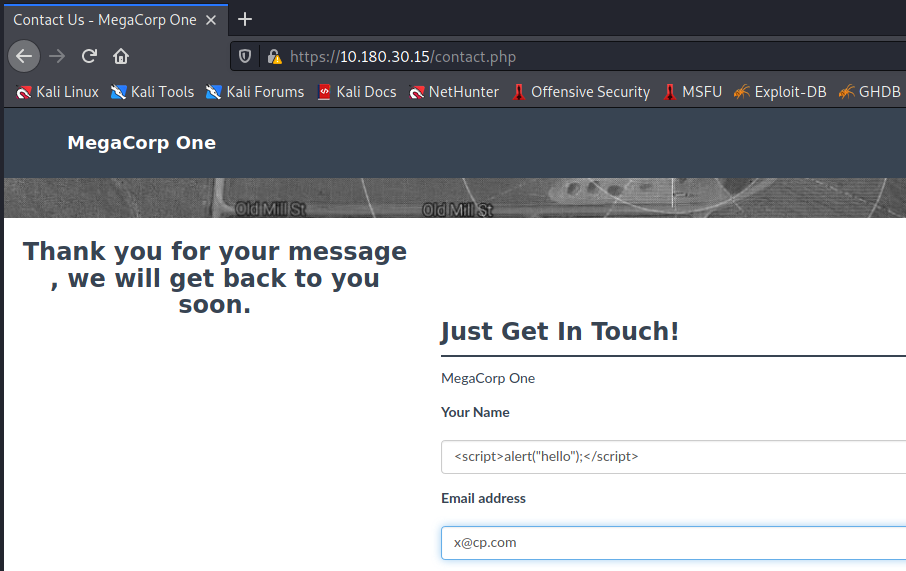
\includegraphics[width=0.99\linewidth]{images/xssattacks-1.png}
    \caption{Page vulnérable à une attaque XSS et payload}
    \label{fig:xssattacks-1}
\end{figure}

\begin{figure}[H]
    \centering
    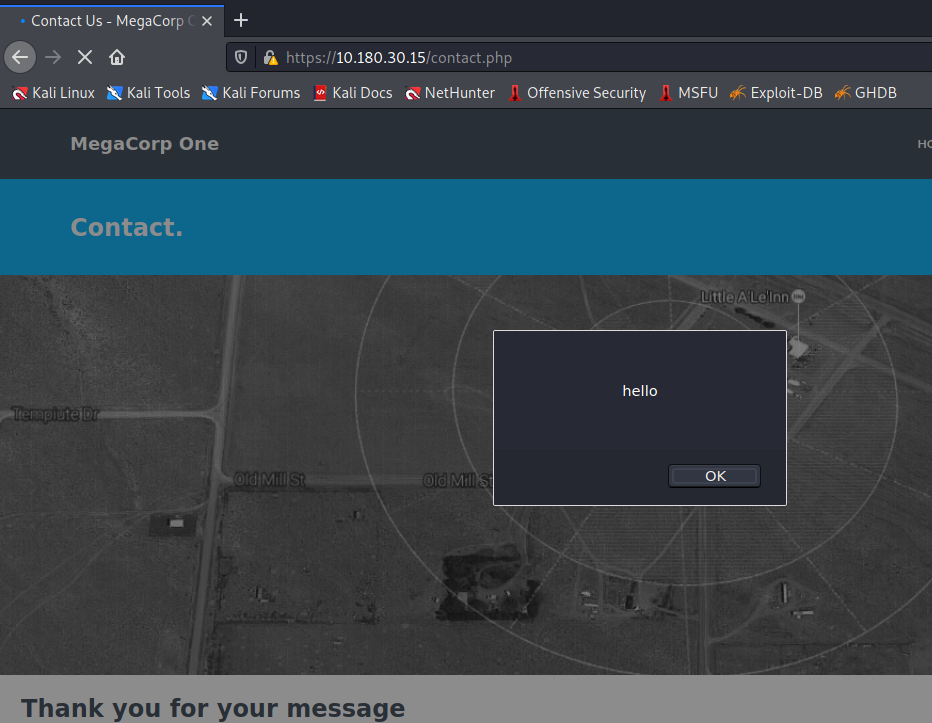
\includegraphics[width=0.75\linewidth]{images/xssattacks-2.png}
    \caption{Résultat de l'attaque XSS}
    \label{fig:xssattacks-2}
\end{figure}


\end{itemize}

\textbf{Information :}\\
\begin{itemize}
    \item Nginx version\\
Nessus à détecté la version de Nginx comme étant la 1.18.0. \\
\end{itemize}



\subsubsection{Analyse web avec l'outil Nikto}

Nous avons également scanné les sites web avec l'outil nikto dont voici les résultats pour chaque hôte:
\begin{itemize}
    \item \texttt{nikto -host=10.180.30.10}:
    \begin{itemize}
        \item Server: Apache/2.4.7 (Ubuntu)
        \item The anti-clickjacking X-Frame-Options header is not present
        \item The X-XSS-Protection header is not defined. This header can hint to the user agent to protect against some forms of XSS
        \item The X-Content-Type-Options header is not set. This could allow the user agent to render the content of the site in a different fashion to the MIME type
        \item No CGI Directories found (use '-C all' to force check all possible dirs)
        \item Server may leak inodes via ETags, header found with file /, inode: 2cf6, size: 5cde79db3e87c, mtime: gzip
        \item Apache/2.4.7 appears to be outdated (current is at least Apache/2.4.37). Apache 2.2.34 is the EOL for the 2.x branch
        \item Allowed HTTP Methods: GET, HEAD, POST, OPTIONS
        \item OSVDB-3233: /icons/README: Apache default file found.
    \end{itemize}
    \item \texttt{nikto -host=10.180.20.1}:
    \begin{itemize}
        \item Server: Microsoft-IIS/10.0
        \item The anti-clickjacking X-Frame-Options header is not present.
        \item The X-XSS-Protection header is not defined. This header can hint to the user agent to protect against some forms of XSS
        \item The X-Content-Type-Options header is not set. This could allow the user agent to render the content of the site in a different fashion to the MIME type
        \item No CGI Directories found (use '-C all' to force check all possible dirs)
        \item Allowed HTTP Methods: OPTIONS, TRACE, GET, HEAD, POST
        \item Public HTTP Methods: OPTIONS, TRACE, GET, HEAD, POST
    \end{itemize}
    \item \texttt{nikto -host=10.180.30.15}:
    \begin{itemize}
        \item Server: nginx/1.18.0
        \item The anti-clickjacking X-Frame-Options header is not present.
        \item The X-XSS-Protection header is not defined. This header can hint to the user agent to protect against some forms of XSS
        \item The X-Content-Type-Options header is not set. This could allow the user agent to render the content of the site in a different fashion to the MIME type
        \item Root page / redirects to: https://10.180.30.15/
        \item No CGI Directories found (use '-C all' to force check all possible dirs)\\
    \end{itemize}
\end{itemize}
Nous remarquons que ces résultats sont en adéquation avec les vulnérabilités énumérées à l'aide de l'outil Nessus.\\
Notamment le clickjacking, nikto précise qu'il s'agit du header servant de protection contre ce type d'attaques qui est désactivé.\\
Mais aussi que les méthodes HTTP sont activées, ce qui confirme que certaines transmission sont faites en clair. Un attaquant peut donc facilement intercepter le trafic et le lire, notamment des mots de passe.










\subsection{Exploitation}



\subsubsection{Accès au réseau Wi-fi}

L'objectif dans ce cas était de récupérer le mot de passe du Wi-fi afin d'avoir un accès interne à cette partie du réseau.
Nous avons utilisé l'outil Wifite, permettant de trouver le mot de passe d'un réseau Wi-fi chiffré, dans notre cas il s'agissait du WPA2.\\

Après le lancement du logiciel sous Kali Linux (voir figure \ref{fig:wifite}).

\begin{figure}[H]
    \centering
    
\includegraphics[width=0.50\linewidth]{images/wifite.png}
    \caption{Lancement de l'outil Wifite}
    \label{fig:wifite}
\end{figure}

Wifite nous proposait différents réseaux wi-fi, nous avons donc sélectionné notre réseau cible. Il s'agit du réseau n°5 \textit{Ikki}.
Finalement, à l'aide de wordlists, le mot de passe correspondant au réseau wi-fi cible à pu être identifié (voir figure \ref{fig:mdpwifi}).

\begin{figure}[H]
    \centering
    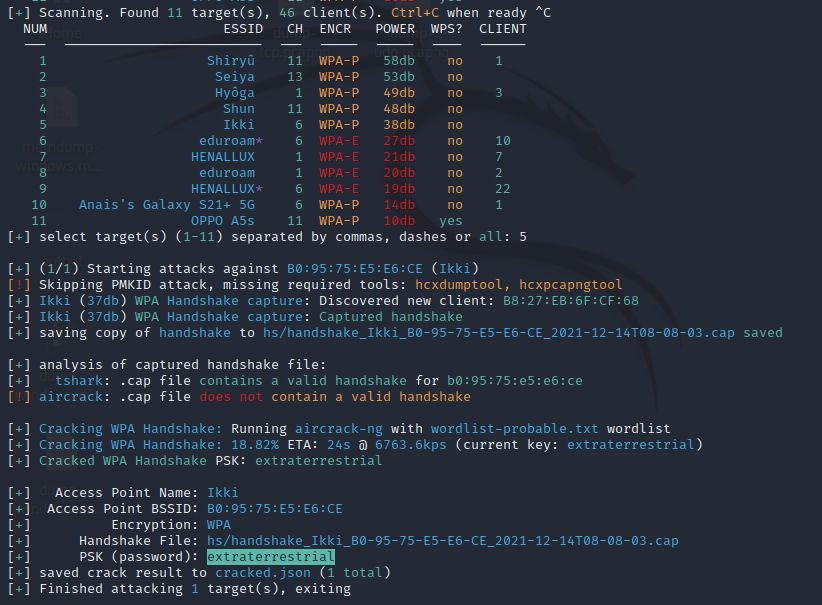
\includegraphics[width=0.99\linewidth]{images/mdpwifi.png}
    \caption{Mot de passe du réseau Wi-fi}
    \label{fig:mdpwifi}
\end{figure}



\subsubsection{Tentative de connexion SSH}

Lors de la phase de reconnaissance, nous avions trouvé les combinaisons de noms d'utilisateurs et mots de passe suivants:
\begin{itemize}
    \item trivera - Tanya4life
    \item Wadler - TwitterStar2
\end{itemize}
Le mot de passe de l'utilisateur \textit{trivera} avait pu être facilement trouvé à l'aide du hash présent sur le github du site web ainsi que de l'outil \textit{JohnTheRipper} et de la liste publique \textit{rockyou.txt}.\\
Nous avons tentés d'effectuer une connexion ssh sur les adresses suivantes: 10.180.20.1 - 10.180.20.2 - 10.180.20.3 - 10.180.30.10 - 10.180.30.15\\
Cependant, nous n'avons pas réussi à exploiter ces identifiants. C'est un point positif car nous aurions pu avoir accès facilement aux systèmes de l'entreprise.



\subsubsection{Tentative d'exploitation par une faille CVE}

La version d'Apache sur la machine 10.180.30.10 n'est pas récente, c'est la version 2.4.7. Or, Apache est déjà arrivé à la version 2.4.51. Étant donné que la version d'Apache utilisée possède des failles, nous avons tentés de les exploiter avec un exploit disponible sur \texttt{exploit-db.com}. Ceci n'a rien donné comme vous pouvez le voir sur la figure \ref{fig:apache-exploit-fail}. Cependant, cela montre que MegaCorpOne doit adopter une politique de mise à jour.

\begin{figure}[H]
    \centering
    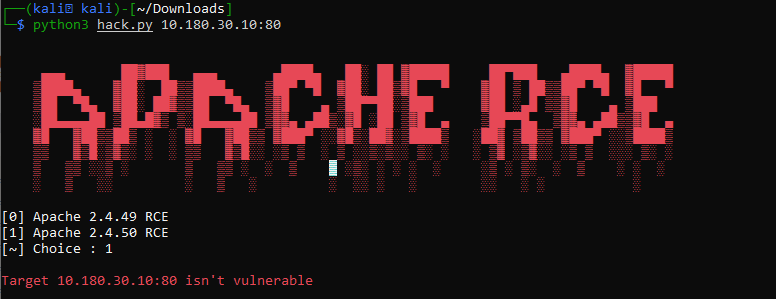
\includegraphics[width=15cm]{images/apache-exploit-fail.png}
    \caption{Tentative d'exploitation d'Apache via les CVE 2021-42013 et 2021-41773}
    \label{fig:apache-exploit-fail}
\end{figure}



\subsubsection{Connexion Wordpress}

À l'aide de Nessus, lors de la phase de scanning, nous avons pu obtenir des noms d'utilisateurs pour la partie Wordpress du site web. Le nom d'utilisateur blogger correspond également au mot de passe de ce même utilisateur.\\
Avec les identifiants \textit{blogger/blogger}, nous pouvons donc accéder à l'interface de management de Wordpress (figure \ref{fig:wordpress-admin}). Comme le plugin \textit{slideshow-gallery} autorise l'upload de tout type de fichier, y compris PHP, nous pouvons mettre un payload reverse shell pour obtenir un accès directement à la machine (figures \ref{fig:wordpress-upload} et \ref{fig:shell-php}).

\begin{figure}[H]
    \centering
    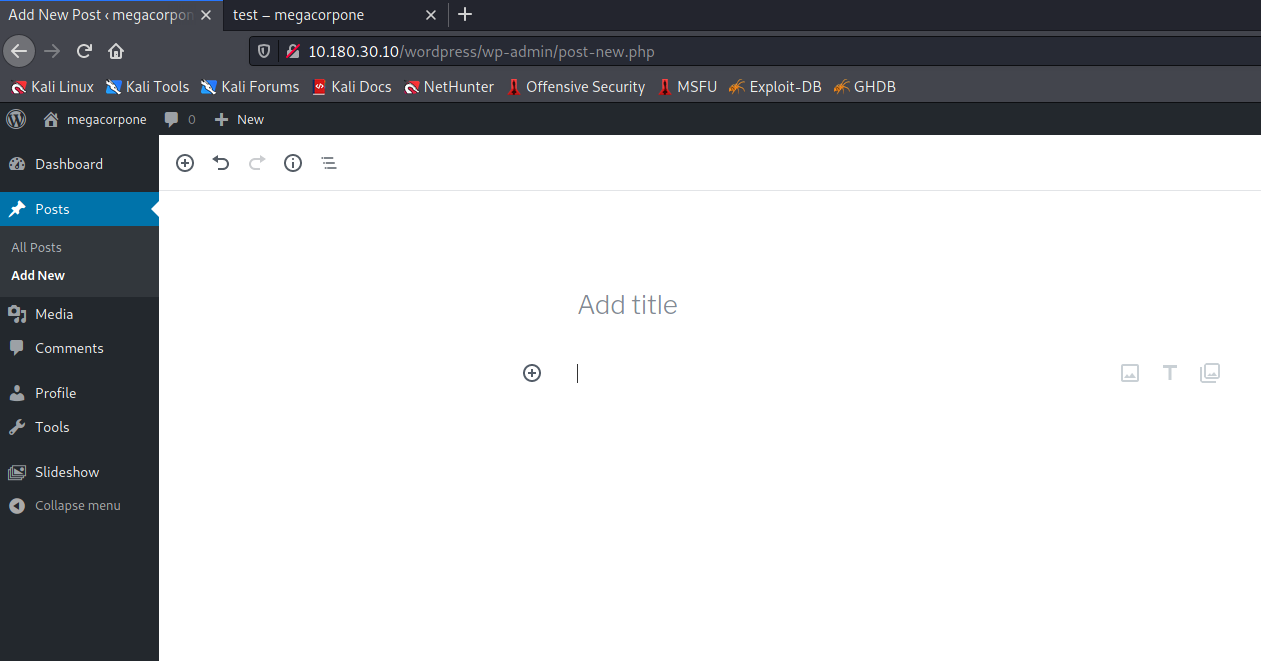
\includegraphics[width=0.99\linewidth]{images/wordpress-admin.png}
    \caption{Interface d'administration de Wordpress}
    \label{fig:wordpress-admin}
\end{figure}

\begin{figure}[H]
    \centering
    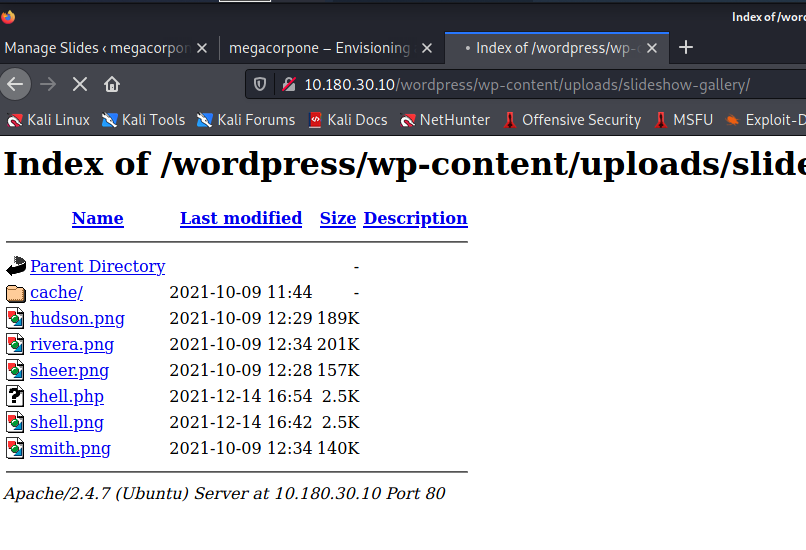
\includegraphics[width=0.65\linewidth]{images/wordpress-upload.png}
    \caption{Upload d'une reverse shell PHP}
    \label{fig:wordpress-upload}
\end{figure}

\begin{figure}[H]
    \centering
    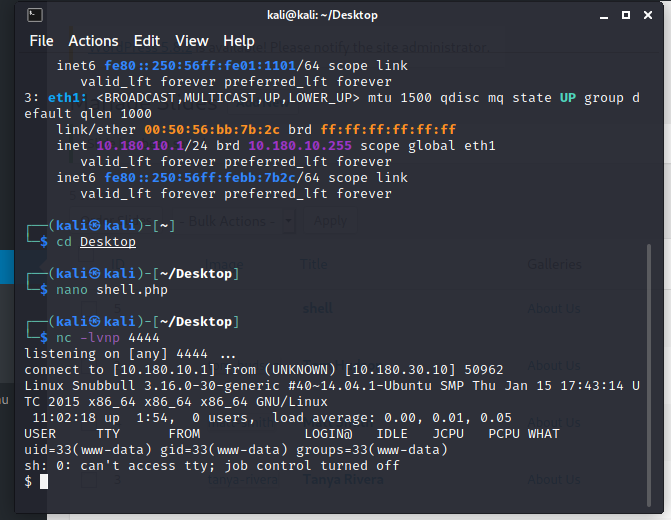
\includegraphics[width=0.70\linewidth]{images/shell-php.png}
    \caption{Obtention d'un accès shell à la machine 10.180.30.10}
    \label{fig:shell-php}
\end{figure}



\subsubsection{Brute force des identifiants et accès aux shares}

Sur la figure \ref{fig:smbaccess}, vous pouvez voir que nous avons réussi à obtenir un accès authentifié aux shares smb. Ces dossiers partagés ont pu être trouvé à l'aide du scan nessus et Nmap effectué plus tôt (voir \ref{fig:smb-shares-enum-msf} et \ref{fig:sharefolder}). Grâce aux énumérations des utilisateurs effectuées plus tôt avec Nmap (voir \ref{fig:snmpwalk}, nous avons obtenu une liste de comptes utilisateurs existants sur la machine. De plus, dans le dossier partagé \textit{GitHub\$} se trouvait le fichier \textit{ptlab\_leakpasswords.txt}. Il s'agit d'une liste de mots de passe. A l'aide du module \textit{auxiliary/scanner/smb/smb\_login}, nous avons pu utilisé cette liste de mot de passe ainsi que la liste d'utilisateurs que nous possédions pour trouver une combinaison d'identifiants: \texttt{winxp - P@55w0rd!}(fig \ref{fig:winxppassword}). Et ainsi obtenir un accès plus important (fig \ref{fig:smbaccess}).\\

Sur la figure \ref{fig:smbaccess} la commande utilisée retourne le résultat dans le dossier /mnt de notre machine.
Les options -o username et password sont utilisées afin de spécifier les identifiants à utilisés pour obtenir l'accès au dossier partagé demandé.

\begin{figure}[H]
    \centering
    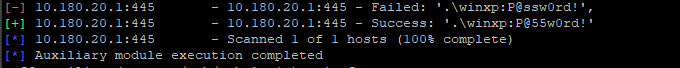
\includegraphics[width=0.99\linewidth]{images/password_winxp.png}
    \caption{Mot de passe de l'utilisateur Winxp}
    \label{fig:winxppassword}
\end{figure}

\begin{figure}[H]
    \centering
    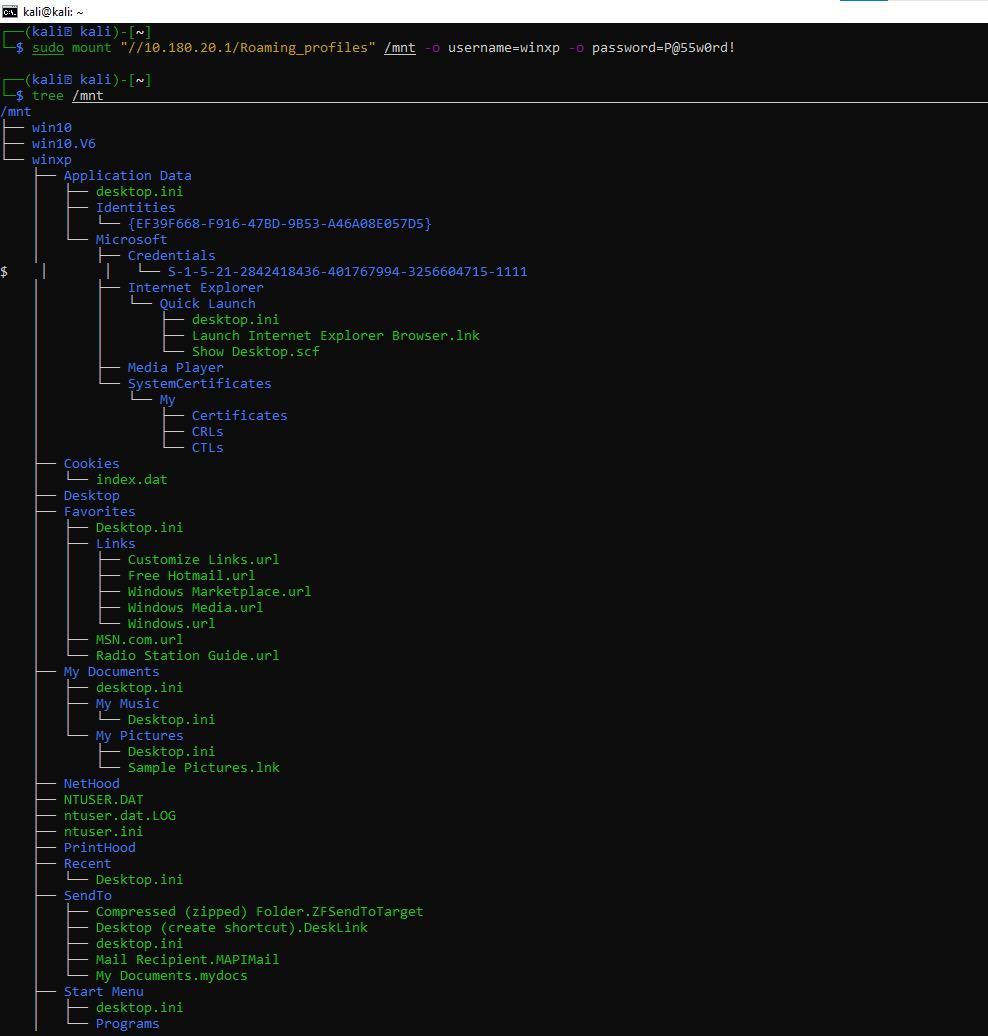
\includegraphics[width=0.99\linewidth]{images/smb-access.png}
    \caption{Accès aux shares après brute force des mots de passe}
    \label{fig:smbaccess}
\end{figure}



\subsubsection{Exécutions de commandes via le service SMB}

Comme le service SMB de la machine Windows XP qui possède l'adresse IP 10.180.20.2 est une version ancienne, elle possède de nombreuse failles qui peuvent être exploitées. Parmi celles-ci, nous comptons notamment la \textit{CVE-2017-0143} aussi connue sous le nom d'\textit{EternalBlue}. C'est une vulnérabilité critique parce qu'elle permet une exécution de code à distance. Pour l'exploiter, nous pouvons compter sur le module \textit{auxiliary/smb/ms17\_010\_command} de metasploit. Vous pouvez voir l'exécution de la commande \texttt{whoami}, qui affiche l'identité de l'utilisateur lançant la commande, sur la figure \ref{fig:smbexploit}. L'utilisateur est: \texttt{nt authority$\backslash$system} qui possède des privilèges administrateur.\\
Les paramètres à utiliser sont:
\begin{itemize}
    \item RHOST = l'IP de la machine cible
    \item COMMAND = Commande à exécuter sur la machine cible
\end{itemize}

\begin{figure}[H]
    \centering
    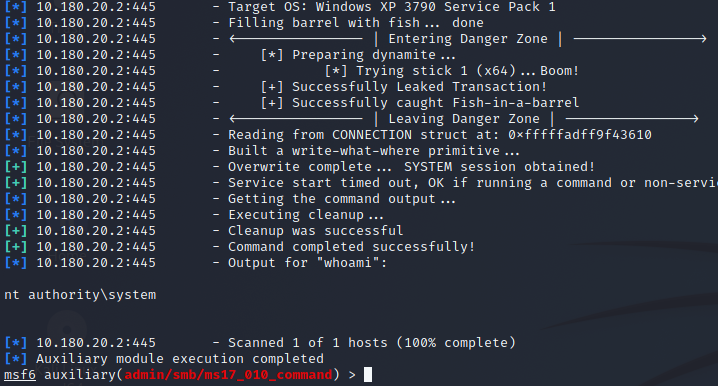
\includegraphics[width=0.80\linewidth]{images/smb-exploit.png}
    \caption{Exploitation de la faille EternalBlue sur la machine 10.180.20.2}
    \label{fig:smbexploit}
\end{figure}



\subsubsection{Ouverture d'un shell meterpreter via le service SMB}

Suite à la découverte de la faille EternalBlue, nous avons tenté d'ouvrir un shell sur la machine. C'est ce que nous avons fait sur la figure \ref{fig:smbexploit2} à l'aide du module \textit{windows/smb/ms17 010 psexec}. Une fois que c'est réalisé, nous pouvons facilement faire sortir des données confidentielles, obtenir un accès à l'interface graphique (fig \ref{fig:smbexploit3}) créer de nouveaux comptes utilisateurs pour maintenir un accès au système, etc. Cependant, nous ne sommes administrateurs que sur une seule machine et notre objectif va désormais être d'étendre notre emprise sur d'autres machines au sein du réseau de MegaCorpOne. C'est ce qu'on appelle le mouvement latéral.

\begin{figure}[H]
    \centering
    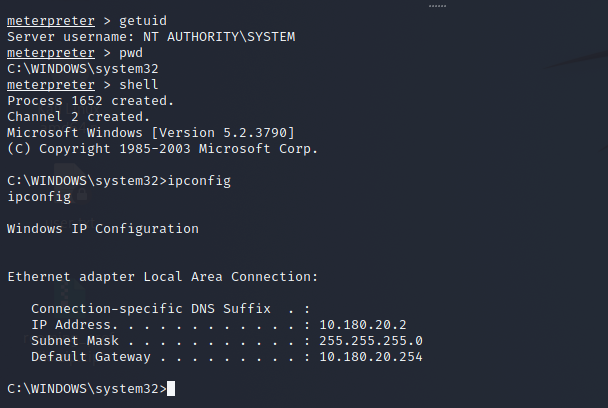
\includegraphics[width=0.70\linewidth]{images/smb-exploit2.png}
    \caption{Ouverture d'un shell meterpreter sur la machine 10.180.20.2}
    \label{fig:smbexploit2}
\end{figure}

Sur l'image ci-dessous (figure \ref{fig:smbexploit3}), nous avons créer un utilisateur via notre accès shell et nous accédons à cet utilisateur à l'aide du protocole RDP afind d'avoir un accès à l'interface graphique.

\begin{figure}[H]
    \centering
    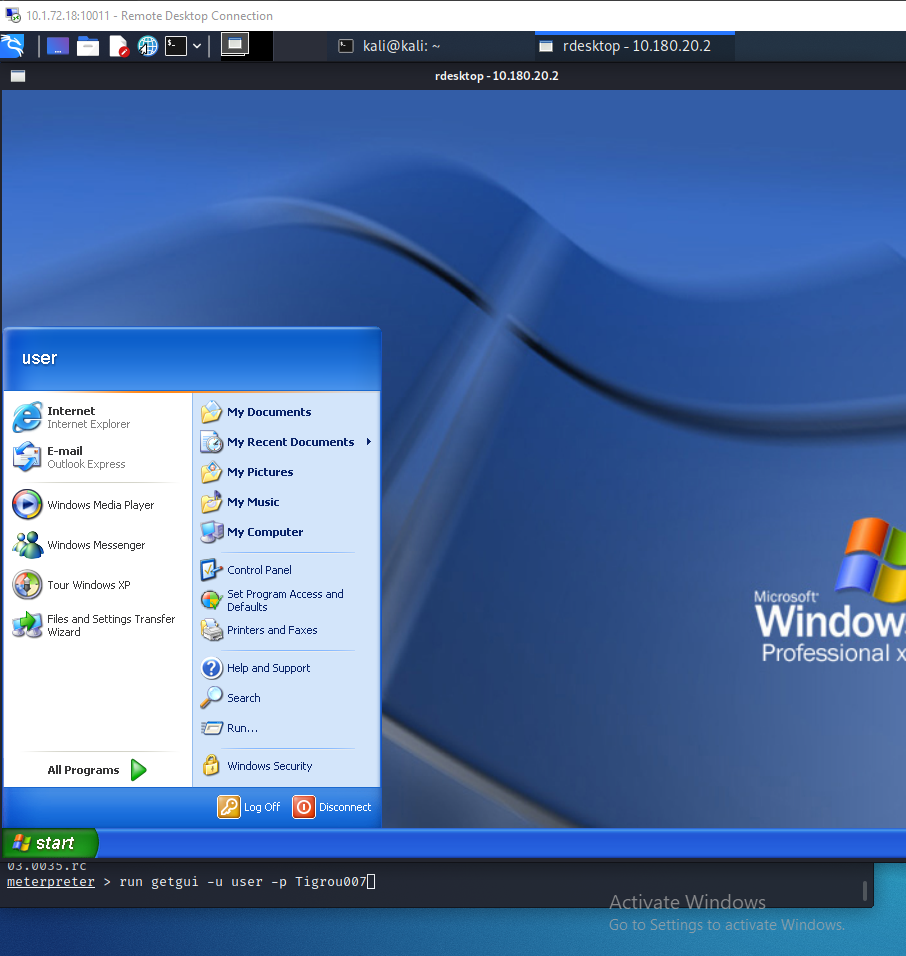
\includegraphics[width=0.80\linewidth]{images/smb-exploit3.png}
    \caption{Ouverture de l'interface graphique sur la machine 10.180.20.2}
    \label{fig:smbexploit3}
\end{figure}










\subsection{Élévation de privilèges}

Dans ce cas ci, l'élévation de privilèges ne va concerner que la machine 10.180.30.10 sur laquelle nous avons pu obtenir un accès shell non-privilégié (figure \ref{fig:shell-php}). En effet, l'élévation de privilège au sein de l'Active Directory va se faire en même temps que le mouvement latéral et sera donc couvert dans cette section du rapport.

L'élévation de privilèges sur cette machine fut très simple. En effet, à cause d'une configuration sudo, permettant à l'utilisateur www-data de lancer l'exécutable strace sans mot de passe avec les privilèges root (figure \ref{fig:sudo-1}), nous avons pu obtenir un shell avec l'utilisateur root comme vous pouvez le voir sur la figure \ref{fig:sudo-2}.

\begin{figure}[H]
    \centering
    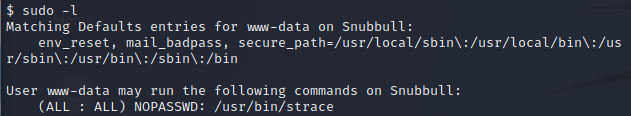
\includegraphics[width=0.70\linewidth]{images/sudo-l.png}
    \caption{Permissions sudo de l'utilisateur www-data sur la machine 10.180.30.10}
    \label{fig:sudo-1}
\end{figure}

\begin{figure}[H]
    \centering
    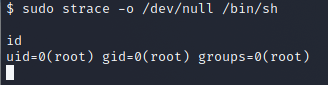
\includegraphics[width=0.50\linewidth]{images/sudo-strace.png}
    \caption{Élévation de privilèges sur la machine 10.180.30.10}
    \label{fig:sudo-2}
\end{figure}










\subsection{Mouvement latéral}

Nous avons pu obtenir le hash d'un mot de passe d'un compte privilégié avec la méthode Kerberoast (figure \ref{fig:kerberoast}). Ensuite, nous l'avons testé contre des listes de mots de passe pour le retrouver (figure \ref{fig:crackpassword}). Une fois que nous avons trouvé le mot de passe, nous avons pu nous connecter avec ces identifiants en RDP sur la machine 10.180.20.3 (figure \ref{fig:lateral1}), puis les réutiliser pour nous connecter en RDP vers le point central de l'Active Directory, le serveur 10.180.20.1 (figure \ref{fig:lateral2}). Maintenant que nous sommes connectés avec un compte administrateur de l'Active Directory sur le serveur central, nous avons effectivement compromis l'infrastructure informatique de MegaCorpOne.

\begin{figure}[H]
    \centering
    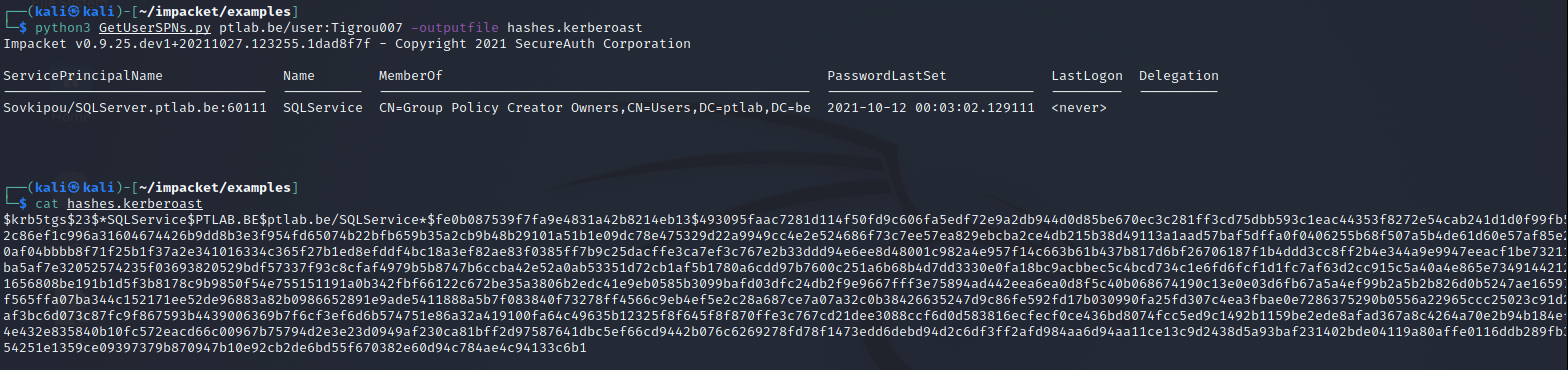
\includegraphics[width=0.99\linewidth]{images/hashes-kerberoast.png}
    \caption{Obtention du hash d'un mot de passe d'un compte privilégié avec la méthode Kerberoast}
    \label{fig:kerberoast}
\end{figure}

\begin{figure}[H]
    \centering
    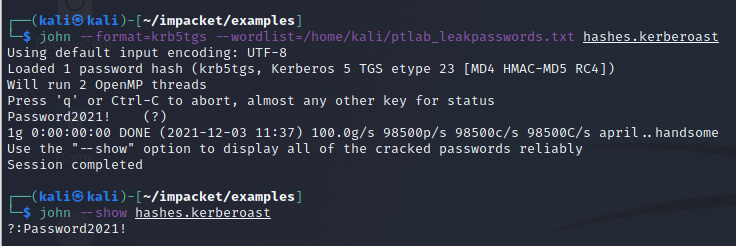
\includegraphics[width=0.90\linewidth]{images/crack-password.png}
    \caption{Crack du hash du mot de passe avec \texttt{john}}
    \label{fig:crackpassword}
\end{figure}

\begin{figure}[H]
    \centering
    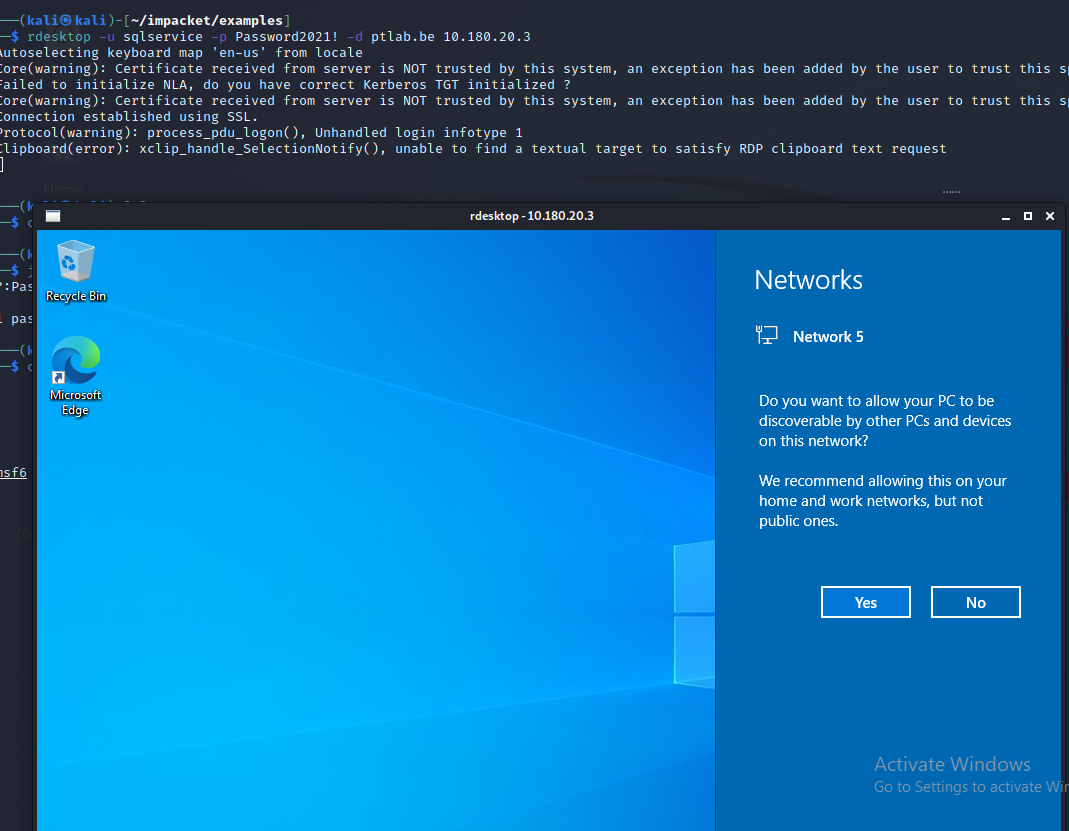
\includegraphics[width=0.90\linewidth]{images/lateral1.png}
    \caption{Déplacement latéral vers la machine 10.180.20.3}
    \label{fig:lateral1}
\end{figure}

\begin{figure}[H]
    \centering
    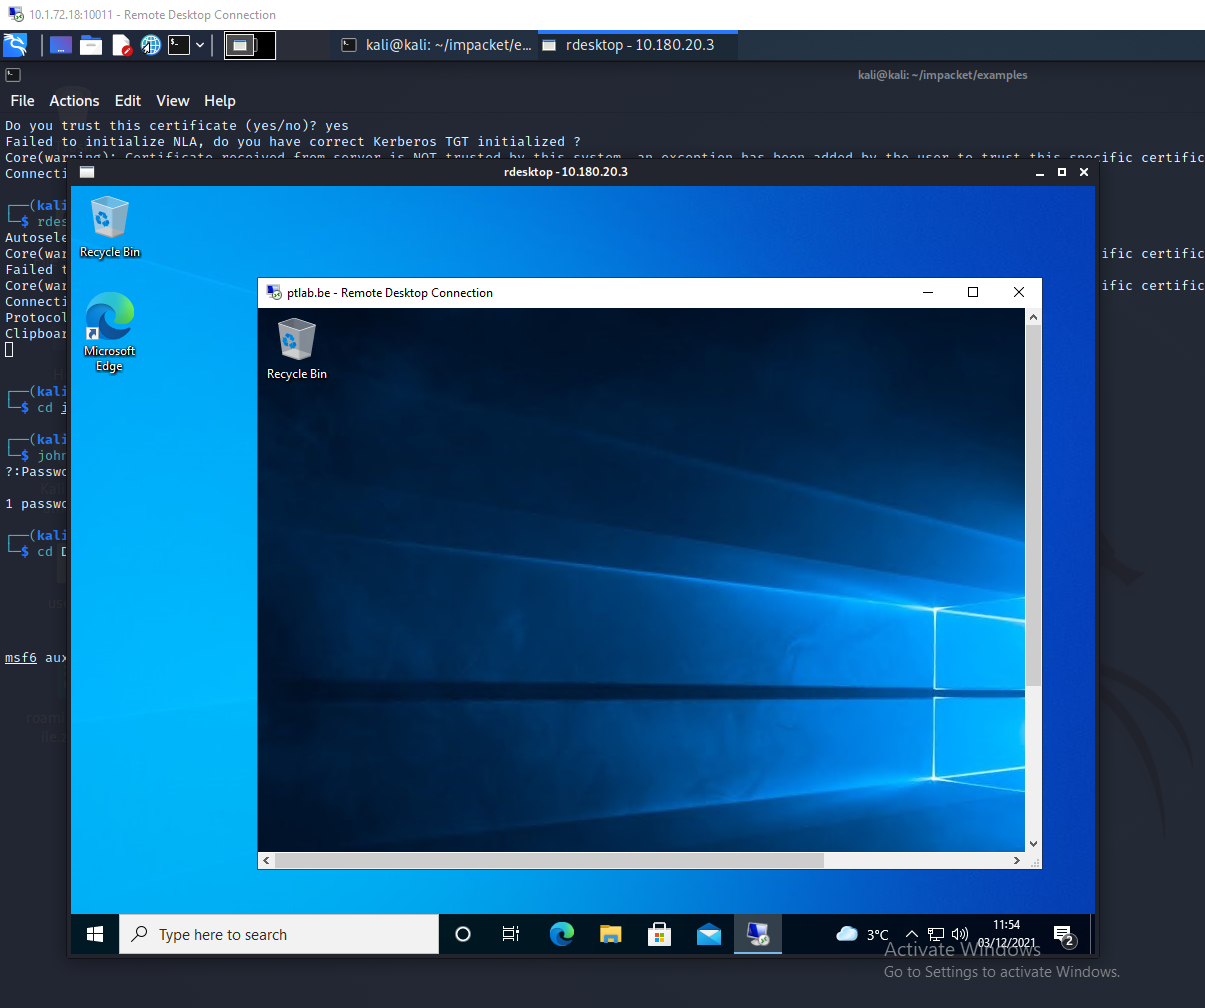
\includegraphics[width=0.90\linewidth]{images/lateral2.png}
    \caption{Déplacement latéral vers le serveur contenant l'Active Directory: 10.180.20.1}
    \label{fig:lateral2}
\end{figure}



\subsubsection{Scan depuis l'intérieur de l'infrastructure}

A l'aide de notre accès RDP au compte de l'utilisateur SQLService sur la machine WindowsServer, nous avons pu réaliser un scan de vulnérabilités depuis l'intérieur de l'infrastructure.\\
\begin{itemize}
    \item A l'adresse 10.180.20.1, la faille la plus critique trouvée est le manque de plusieurs mises à jour de sécurité pour le système d'exploitation. Ce qui expose la machine à de multiples vulnérabilités.
    \item La version du logiciel VMWare Tools installée est affectée par une vulnérabilité locale d'escalation de privilèges et une vulnérabilité DOS.
    \item Le disque C: est partagé via le service SMB.
\end{itemize}



\subsection{Recommandations de sécurité} \label{mesures}

\begin{itemize}

\item En ce qui concerne le réseau Wi-fi:
\begin{itemize}
    \item [\textbullet] Mise en place d'un portail de connexion pour les invités, clients, ...
    \item [\textbullet] Utiliser un mot de passe fort
    \item [\textbullet] Mise en place d'un pare-feu\\
\end{itemize}

\item Différentes failles sont présentes concernant les mots de passe. Ils sont affichés sur une photo, ils peuvent être déchiffrés facilement, des éléments pouvant aider à les déchiffrer sont trouvables facilement.\\
Nous recommandons d'établir au sein de l'entreprise:
\begin{itemize}
    \item [\textbullet]Une politique de sécurité des mots de passe\\
\end{itemize}

\item Des fichiers sensibles sont présents dans des dossiers partagés. Ces fichiers doivent être supprimés ou isolés du système de l'entreprise afin de de ne pas être découvert par un attaquant.\\

\item Le service SMB doit être sécurisé :
\begin{itemize}
    \item [\textbullet]S'assurer que les mots de passe sont envoyés de manière chiffrée
    \item [\textbullet]Protéger les ressources par un mot de passe
    \item [\textbullet]Ne pas laisser un accès libre aux shares
    \item [\textbullet] Mise à jour de la version \\
\end{itemize}

\item Les systèmes d'exploitation utilisés sur les différentes machines contiennent de nombreuses vulnérabilités et ne sont parfois plus soumis à des mises à jour de sécurité. L'entreprise doit envisager un passage à une version supérieur du système.\\

\item L'upload de fichiers sur l'interface d'administration de Wordpress doit être restreinte pour qu'on ne puisse pas uploader des fichiers PHP permettant par la suite d'exécuter du code et obtenir un accès au système. \\

\item Changement des configurations sudo pour éviter qu'un utilisateur puisse lancer un exécutable sans mot de passe avec des permissions root. \\

\item Mise en place d'un anti-virus sur les machines. 

\end{itemize}










\cleardoublepage
\newpage


\section{Conclusion}

Pour conclure, l'infrastructure de la société MegaCorpOne est fortement vulnérable à différents types d'attaques. Nous avons pu récolter de nombreuses informations tout au long de ce test de pénétration, qui nous ont permis d'accéder à l'intérieur du système. Des informations sensibles sont d'ailleurs accessibles facilement depuis l'extérieur.

La société doit adopter de nouvelles mesures afin de renforcer sa sécurité. Différentes mesures jugées importantes, suite aux différents scans et exploitations menées, sont déjà répertoriées dans la section \textit{\ref{mesures} Recommandations de sécurité}.

Nous conseillons de suivre ces recommandations et de mettre en place ces mesures. Mais aussi, de continuer par la suite à améliorer et sécuriser le système afin d'éviter tout type d'attaque.

























\appendix \newpage

























\section{Scan TCP}

Il y a deux manières de faire un scan TCP:
\begin{itemize}
    \item envoyer un paquet SYN et attendre une réponse SYN-ACK pour voir si le port est ouvert,
    \item créer une connexion TCP complète.
\end{itemize}

On peut tester la seconde option facilement avec la commande suivante: \texttt{nc -nvv -w 1 -z 10.180.20.1 3388-3390}, dont voici le résultat:
\begin{example}
\begin{Verbatim}
(UNKNOWN) [10.180.20.1] 3390 (?) : Connection timed out
(UNKNOWN) [10.180.20.1] 3389 (ms-wbt-server) open
(UNKNOWN) [10.180.20.1] 3388 (?) : Connection timed out
\end{Verbatim}
\end{example}

Les options de la commande permettent:
\begin{itemize}
    \item -n (numeric-only) : Prend en charge uniquement les IP et pas les noms de DNS
    \item -v : Permet une sortie détaillée (utilisé en double permet une sortie encore plus détaillée)
    \item -w : Permet de définir des délais d'inactivité
    \item -z : Mode scan de port, uniquement les services qui écoutent seront scannés
\end{itemize}

Un port peut être dans trois états différents:
\begin{itemize}
    \item ouvert, il répond positivement au paquet TCP SYN avec un paquet TCP SYN-ACK pour ouvrir la connexion;
    \item fermé, il répond par un message négatif;
    \item filtré, il ne répond pas.
\end{itemize}

Avec une capture wireshark (fig. \ref{fig:scantcp}), on peut observer que les ports 3388 et 3390 sont filtrés parce qu'ils ne répondent pas à nos messages TCP SYN. En revanche, le port 3390 de la machine 10.180.20.1 est bien ouvert parce qu'il ouvre la connexion en terminant la poignée de main TCP.

Comme expliqué précédemment, plutôt que de réaliser une connexion TCP complète, nous pouvons également envoyer seulement le paquet TCP SYN et recevoir la réponse TCP SYN-ACK sans envoyer le troisième paquet (TCP ACK) qui ouvrirait la connexion. Ainsi, certains firewalls ne remarqueront pas que nous essayons de scanner des machines qu'ils sont sensés protéger. Pour le faire, nous devons utiliser l'option nmap \texttt{-sT} et avoir des privilèges administrateur sur la machine.

\begin{figure}[H]
    \centering
    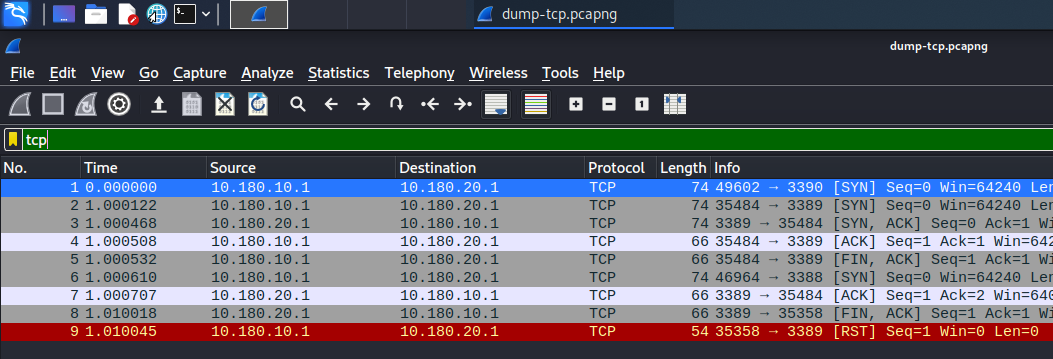
\includegraphics[width=0.95\linewidth]{images/scan-tcp.png}
    \caption{Trafic généré par un scan TCP}
    \label{fig:scantcp}
\end{figure}














\section{Scan UDP}

Nous pouvons réaliser un simple scan UDP avec la commande suivante: \texttt{nc -nv -u -z -w 1 10.180.20.1 160-162}. Cependant avec les scans UDP, il y a une difficulté supplémentaire: le protocole n'envoie pas forcément de réponse quand on envoie un message. Ainsi, sur la figure \ref{fig:scanudp}, on remarque que nos messages restent sans réponses mais le résultat du scan ci-dessous indique que les ports sont ouverts:

\begin{example}
\begin{Verbatim}
(UNKNOWN) [10.180.20.1] 162 (snmp-trap) open
(UNKNOWN) [10.180.20.1] 161 (snmp) open
(UNKNOWN) [10.180.20.1] 160 (?) open
\end{Verbatim}
\end{example}

Les options utilisées sont:
\begin{itemize}
    \item -n (numeric-only) : Prend en charge uniquement les IP et pas les noms de DNS 
    \item -v : Permet une sortie détaillée (utilisé en double permet une sortie encore plus détaillée) 
    \item -u : Permet d'utiliser le mode UDP avec la commande netcat
    \item -w : Permet de définir des délais d'inactivité
    \item -z : Mode scan de port, uniquement les services qui écoutent seront scannés
\end{itemize}

\begin{figure}[H]
    \centering
    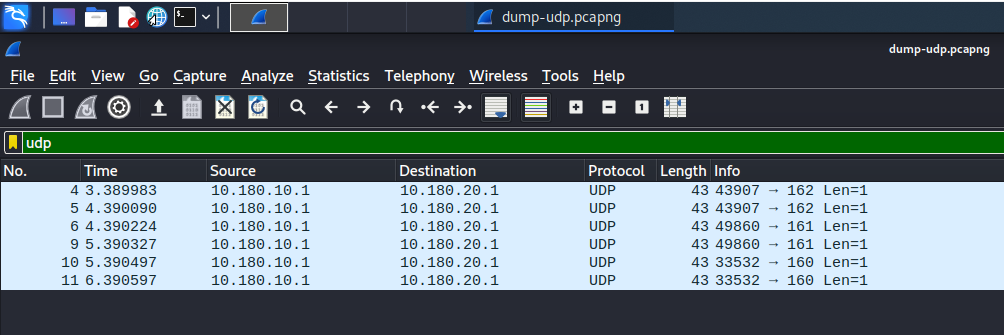
\includegraphics[width=0.90\linewidth]{images/scan-udp.png}
    \caption{Trafic généré par un scan UDP}
    \label{fig:scanudp}
\end{figure}















\section{Quantité de trafic généré par nos scans}

Commandes pour activer le comptage des paquets:
\begin{itemize}
    \item \texttt{sudo iptables -I INPUT 1 -s [ IP ] -j ACCEPT}
    \item \texttt{sudo iptables -I OUTPUT 1 -d [ IP ] -j ACCEPT}
    \item \texttt{sudo iptables -Z}
\end{itemize}

Commande pour visualiser le résultat: \texttt{sudo iptables - vn -L}

Après le scan SYN, effectué avec la commande: \texttt{sudo nmap -sS 10.180.30.15}, nous obtenons:
\begin{example}
\begin{Verbatim}
Chain INPUT (policy ACCEPT 2791 packets, 135K bytes)
 pkts bytes target   prot opt in   out   source         destination
 1004 40172 ACCEPT   all  --  *    *     10.180.30.15   0.0.0.0/0

Chain FORWARD (policy ACCEPT 0 packets, 0 bytes)
 pkts bytes target   prot opt in   out   source         destination

Chain OUTPUT (policy ACCEPT 1345 packets, 6532K bytes)
 pkts bytes target   prot opt in   out   source         destination
 1010 44392 ACCEPT   all  --  *    *     0.0.0.0/0      10.180.30.15
\end{Verbatim}
\end{example}

Après le scan connect, effectué avec la commande: \texttt{sudo nmap -sT 10.180.30.15}, nous obtenons:
\begin{example}
\begin{Verbatim}
Chain INPUT (policy ACCEPT 0 packets, 0 bytes)
 pkts bytes target     prot opt in     out     source               destination 
 1004 40252 ACCEPT     all  --  *      *       10.180.30.15         0.0.0.0/0

Chain FORWARD (policy ACCEPT 0 packets, 0 bytes)
 pkts bytes target     prot opt in     out     source               destination

Chain OUTPUT (policy ACCEPT 0 packets, 0 bytes)
 pkts bytes target     prot opt in     out     source               destination 
 1015 60712 ACCEPT     all  --  *      *       0.0.0.0/0            10.180.30.15
\end{Verbatim}
\end{example}

Nous voyons en comparant les résultats de ces deux scans que les scans TCP SYN génèrent moins de trafic que ceux qui font la poignée de main TCP au complet, ce qui est un résultat attendu.















\newpage \listoffigures % \newpage \listoflistings
\newpage
\begin{thebibliography}{9}
\bibitem{1} Consulté le 20-11-2021 \url{https://www.whois.com/whois/megacorpone.com}
\bibitem{2} Consulté le 20-11-2021 \url{https://www.ionos.fr/digitalguide/serveur/outils/netcat/}
\bibitem{3} Consulté le 20-11-2021 \url{https://www.commandlinux.com/man-page/man1/nc.1.html}
% \bibitem{4} 
% \bibitem{5} 
% \bibitem{6} 
\end{thebibliography}




















\end{document}
